\chapter{输运方程}
\label{chap:transport-equations}

往一条缓缓流动的河里滴一滴墨水。如果忽略墨水向周围的扩散，墨迹只是被水流带着走：水流均匀时，它平移；水流越往下游越快时，它被拉长；水流汇聚时，它被压缩。给定水流的速度，我们想算出此后任意时刻、任意位置的墨水情况。

这个问题的答案取决于“墨水情况”指的是什么。假设每个水粒子带着一个标签，比如颜色的编号，那么粒子走到哪里，标签就带到哪里，数值不变。假设我们关心的是单位长度里有多少墨水，事情就不同了：水流把一段河水拉长一倍，同样多的墨水摊在两倍的长度上，浓度减半。同一个流动，同一个初始形状，这两种量的演化规律不同。

本章先讨论第一种量。沿着粒子的轨迹看，偏微分方程退化成常微分方程，第~\ref{chap:ode-sensitivity}章的流映射正好把初始位置和当前位置联系起来。然后由质量平衡推出第二种量满足的方程，并说明两者的差别恰好来自流动造成的体积变化。

这些构造都依赖足够规则的速度场。最后两节讨论初值带间断时方程应当如何理解，以及数据、源项和速度场的误差怎样影响解。全章速度场都是事先给定的，不受被搬运的量影响。

\section{输运问题}
\label{sec:transp-problem}

先看最简单的情形：一条直河以恒定速度$v$向右流动。用$u(x,t)$表示时刻$t$、位置$x$处水粒子携带的量，比如颜色的深浅。粒子不改变自己携带的值，时刻$t$位于$x$的粒子，在时刻$0$位于$x-vt$，所以
\begin{equation}
  u(x,t)=u_0(x-vt),
  \label{eq:transp-translate}
\end{equation}
其中$u_0$是初始分布。

设$u_0$可微，用链式法则计算式~\eqref{eq:transp-translate}的两个偏导数：
\[
  \partial_tu=-v\,u_0'(x-vt),\qquad \partial_xu=u_0'(x-vt).
\]
第一式加上第二式的$v$倍，右端抵消，得到恒定速度的\term{输运方程}（transport equation）
\begin{equation}
  \partial_tu+v\,\partial_xu=0.
  \label{eq:transp-constant}
\end{equation}

这个方程可以用两种视角读。站在岸上盯住固定位置，$\partial_tu$是看到的变化率：上游的值不断流过来，变化率等于$-v\,\partial_xu$。坐在随水漂流的小船上，周围的水相对自己不动，看到的值不变。式~\eqref{eq:transp-constant}说的就是这两种观察彼此一致。

图~\ref{fig:transp-shift}取$v=1$，初值是以$0$为中心、半宽为$1$的三角形。(a)中三个时刻的曲线形状相同，只是向右平移。(b)把同一个解画在$(x,t)$平面上，颜色的深浅沿斜线$x=x_0+t$保持不变，这些斜线就是粒子的轨迹。

\begin{BookInlineFigure}
  \centering
  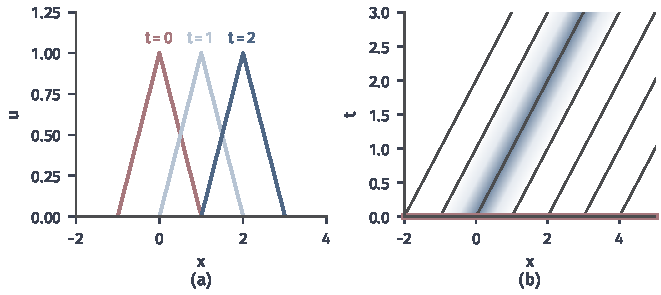
\includegraphics[width=112mm]{figures/06-differential-equations/02-partial-differential-equations/matplotlib/transp-shift/figure.pdf}
  \caption{恒定速度$v=1$的平移。(a)初值（红）和$t=1,2$时的解（蓝色由浅到深）。(b)解$u_0(x-t)$的时空热图，蓝色越深值越大，深灰斜线是粒子轨迹，红线是给定初值的$t=0$。}
  \label{fig:transp-shift}
\end{BookInlineFigure}

水流搬运墨水的比喻有它的边界。真实的墨水还会向四周扩散，边缘逐渐模糊；方程~\eqref{eq:transp-constant}中没有这一项，边缘再陡也不会变缓，初值的尖角和间断都被原样带走。扩散的效果由第~\ref{chap:diffusion-equations}章讨论。

\paragraph{一般的问题}
把水流换成随位置和时间变化的速度场$\bm{v}(\bm{x},t)$，同时允许粒子沿途获得或失去一些量，并考虑有边界的区域，就得到本章要研究的问题。

\begin{definition}[线性输运问题]
\label{def:transp-problem}
设$\Omega\subset\mathbb{R}^{d}$，$\bm{v}:\Omega\times[0,T]\to\mathbb{R}^{d}$是给定的速度场。\term{线性输运问题}（linear transport problem）是求$u(\bm{x},t)$，使
\begin{equation}
  \begin{cases}
    \partial_tu+\bm{v}\cdot\nabla u=f & \text{在}\ \Omega\times(0,T)\ \text{内},\\
    u(\cdot,0)=u_0 & \text{在}\ \Omega\ \text{上},\\
    u=g & \text{在入流边界}\ \Gamma_{-}(t)\ \text{上},
  \end{cases}
  \label{eq:transp-ibvp}
\end{equation}
其中$\bm{n}$是单位外法向，入流边界是
\begin{equation}
  \Gamma_{-}(t)=\{\bm{x}\in\partial\Omega:\bm{v}(\bm{x},t)\cdot\bm{n}(\bm{x})<0\}.
  \label{eq:transp-inflow-boundary}
\end{equation}
当$\Omega=\mathbb{R}^{d}$时，没有边界条件。
\end{definition}

方程中四个已知量的角色不同。
\begin{itemize}
  \item 速度场$\bm{v}$决定粒子往哪里走，它不携带任何场值。
  \item 初始场$u_0$给出时刻$0$在区域内的粒子所携带的值。
  \item 入流数据$g$给出后来从边界进入区域的粒子所携带的值。
  \item 源项$f$描述粒子沿途携带值的变化率，$f=1$表示每个粒子携带的值每单位时间增加$1$。
\end{itemize}

\paragraph{反向追踪}
某个时空点的值由哪些数据决定？从这一点出发，沿粒子的轨迹逆时间往回走，走到已知数据为止。下面以$\Omega=(0,1)$、$v=1/2$为例，此时入流边界只有左端点$x=0$。

如图~\ref{fig:transp-trace}(a)，从$P=(0.8,1)$往回走，轨迹是斜率固定的直线，时间退回$1$时，位置退回$0.5$，到达$(0.3,0)$，落在初始线上。从$Q=(0.2,1)$往回走，在退回时间$0.4$时已到达左端点$(0,0.6)$，落在入流边界上。没有源项时，这两点的值分别是
\[
  u(0.8,1)=u_0(0.3),\qquad u(0.2,1)=g(0.6).
\]

一般地，$(0,1)\times(0,T)$内的点$(x,t)$按下面的方式分成两类，由此得到解的表达式：
\begin{equation}
  u(x,t)=
  \begin{cases}
    u_0(x-vt), & x>vt,\\
    g(t-x/v), & x<vt.
  \end{cases}
  \label{eq:transp-inflow-solution}
\end{equation}
分界线$x=vt$是从角点$(0,0)$出发的轨迹。

\begin{BookInlineFigure}
  \centering
  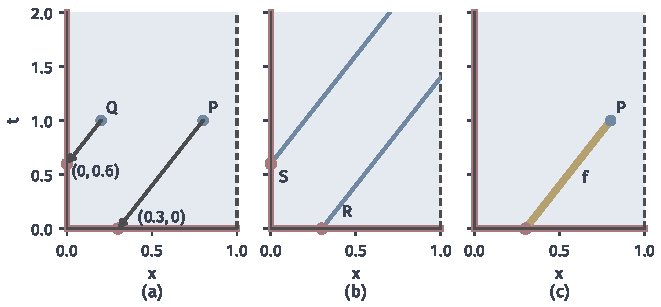
\includegraphics[width=112mm]{figures/06-differential-equations/02-partial-differential-equations/matplotlib/transp-trace/figure.pdf}
  \caption{区间$(0,1)$上$v=1/2$的追踪，红线是给数据的初始线和入流边界，深灰虚线是不给数据的出流边界。(a)从$P,Q$反向追踪到红线上的点。(b)从数据点$R,S$正向出发的影响范围（蓝线）。(c)有源项时，$P$的值还依赖黄色线段上的$f$。}
  \label{fig:transp-trace}
\end{BookInlineFigure}

\paragraph{正向追踪}
反过来，某个数据点影响哪些时空点？从数据点出发沿时间正向走即可。图~\ref{fig:transp-trace}(b)中，从$R$出发的影响范围只有一条线段，这条线段碰到右端点就离开了区域。这与第~\ref{chap:diffusion-equations}章的热方程很不一样，那里一点的扰动瞬间影响全局；与第~\ref{chap:wave-equations}章的波动方程也不同，那里一维的扰动沿左右两条线传播。

\paragraph{源项沿路径累积}
有源项时，粒子沿途不断获得新的量，$P$的值不只依赖轨迹的起点，还依赖整条轨迹上的$f$。如图~\ref{fig:transp-trace}(c)，黄色线段上每一处的$f$都对$u(P)$有贡献，而线段之外的$f$没有影响。这一累积的准确公式在第~\ref{sec:transp-characteristics}节给出。

\paragraph{入流数据与初值的衔接}
式~\eqref{eq:transp-inflow-solution}在分界线$x=vt$的两侧由不同的数据决定，解是否连续取决于角点上的相容性。图~\ref{fig:transp-inflow-solution}比较了两组数据。

(a)中$u_0=\tfrac12(1+\cos2\pi x)$，$g=\cos^{2}(\pi t/2)$。角点上$u_0(0)=g(0)=1$，解沿分界线连续。这里两侧的一阶导数也衔接，因为$u_0'(0)=g'(0)=0$。(b)中$u_0=0$，$g=1$，角点的值不一致，解在分界线上有一个高度为$1$的跳跃，并且这个跳跃沿分界线传播下去，不会被抹平。

\begin{BookInlineFigure}
  \centering
  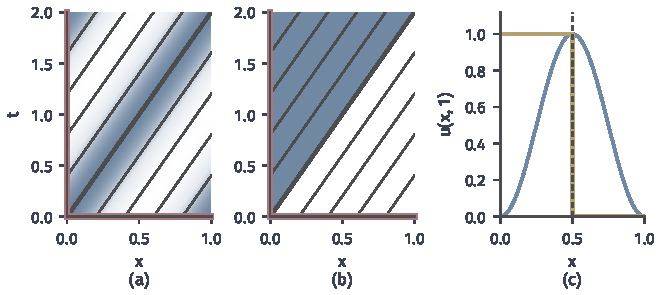
\includegraphics[width=112mm]{figures/06-differential-equations/02-partial-differential-equations/matplotlib/transp-inflow-solution/figure.pdf}
  \caption{$(0,1)$上$v=1/2$的解。(a)初值和入流相容，(b)初值$0$、入流$1$不相容。粗深灰线是分界线$x=t/2$，细深灰线是特征线，红线是给数据的边界，蓝色越深值越大。(c)$t=1$时的剖面，蓝线对应(a)，黄线对应(b)，虚线是分界线的位置。}
  \label{fig:transp-inflow-solution}
\end{BookInlineFigure}

右端点是出流边界，那里的值已由式~\eqref{eq:transp-inflow-solution}确定，不能再独立规定。图~\ref{fig:transp-inflow-solution}(b)的解在$x<t/2$处恒为$1$，在$x>t/2$处恒为$0$，它在分界线上不可导，方程不能逐点成立。这种解的含义留到第~\ref{sec:transp-weak}节讨论。

\section{特征线法}
\label{sec:transp-characteristics}

速度随位置变化时，粒子的轨迹不再是直线，上一节的公式也就不能直接使用。但“坐在小船上看”的想法仍然有效：沿粒子的轨迹求$u$的变化率，偏微分方程会变成常微分方程。

设曲线$\bm{x}(t)$满足$\dot{\bm{x}}=\bm{v}(\bm{x},t)$。沿这条曲线对$u(\bm{x}(t),t)$求导，由链式法则，
\begin{equation}
  \frac{\mathrm{d}}{\mathrm{d}t}u\bigl(\bm{x}(t),t\bigr)
  =\bigl(\partial_tu+\bm{v}\cdot\nabla u\bigr)\bigl(\bm{x}(t),t\bigr).
  \label{eq:transp-along}
\end{equation}
右端正是输运方程的左端。算子$\partial_t+\bm{v}\cdot\nabla$表示跟随粒子时的变化率，称为\term{物质导数}（material derivative）。

\begin{definition}[特征线]
\label{def:transp-characteristic}
设$\bm{v}$是给定的速度场。常微分方程
\begin{equation}
  \dot{\bm{x}}(t)=\bm{v}\bigl(\bm{x}(t),t\bigr)
  \label{eq:transp-char}
\end{equation}
的解$\bm{x}(t)$在时空中的图像$\{(\bm{x}(t),t)\}$称为输运方程的\term{特征线}（characteristic curve）。
\end{definition}

几何上，特征线是时空向量场$(\bm{v},1)$的积分曲线。图~\ref{fig:transp-chardir}中，$(\bm{v},1)$是特征线的切向量，物质导数是$u$沿这个时空方向的方向导数。输运方程规定的只是这一个方向上的导数，其他方向的导数方程不管。这就是沿特征线可以逐条求解的原因。

\begin{BookInlineFigure}
  \centering
  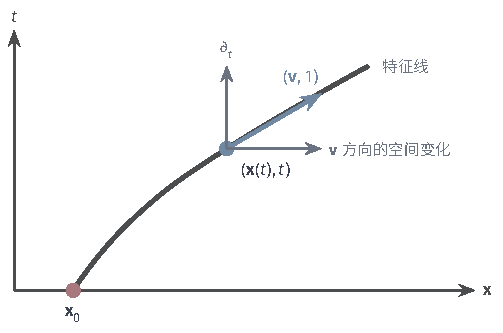
\includegraphics[width=85.2mm]{figures/06-differential-equations/02-partial-differential-equations/tikz/transp-chardir/figure.pdf}
  \caption{时空中的特征线（深灰）。红点是初始位置，蓝色箭头$(\bm{v},1)$是切向量，它由时间方向的一个单位和空间方向的$\bm{v}$合成。物质导数是$u$沿这一方向的方向导数。}
  \label{fig:transp-chardir}
\end{BookInlineFigure}

把偏微分方程沿特征线化为常微分方程，从而逐条求解的方法称为\term{特征线法}（method of characteristics）。

\paragraph{无源输运}
当$f=0$时，式~\eqref{eq:transp-along}说明$u$沿特征线不变。求某点$(\bm{x},t)$的值分三步：解方程~\eqref{eq:transp-char}，得到过这一点的特征线；沿特征线退回到$t=0$，得到出发位置$\bm{x}_0$；令$u(\bm{x},t)=u_0(\bm{x}_0)$。

\begin{example}[均匀拉伸的速度场]
\label{ex:transp-stretch}
取一维速度场$v(x)=x$，初值是以$1$为中心、半宽为$1$的三角形：
\begin{equation}
  u_0(x)=\max\{0,\ 1-\lvert x-1\rvert\}.
  \label{eq:transp-tent}
\end{equation}

特征线满足$\dot{x}=x$，从$x_0$出发的解是
\[
  x(t)=x_0\mathrm{e}^{t}.
\]
反解出发位置，$x_0=x\mathrm{e}^{-t}$。沿特征线$u$不变，于是
\[
  u(x,t)=u_0\bigl(x\mathrm{e}^{-t}\bigr).
\]

在可微的点上代入验证。两个偏导数分别是
\[
  \partial_tu=-x\mathrm{e}^{-t}u_0'\bigl(x\mathrm{e}^{-t}\bigr),\qquad
  x\,\partial_xu=x\mathrm{e}^{-t}u_0'\bigl(x\mathrm{e}^{-t}\bigr),
\]
两者之和为零。

现在算一个具体的点$(x,t)=(3,\ln2)$。特征线的出发位置是$3\mathrm{e}^{-\ln2}=1.5$，所以
\[
  u(3,\ln2)=u_0(1.5)=1-0.5=0.5.
\]
\end{example}

图~\ref{fig:transp-curved}(a)画出了这个例子的特征线。越往右，粒子跑得越快，等间距出发的特征线逐渐散开，解的颜色沿每条特征线不变。(b)是同一个解的剖面：三角形的底从$[0,2]$拉长到$[0,4]$，高度仍然是$1$。(a)中标出的那条特征线把$(1.5,0)$的值$0.5$带到了$(3,\ln2)$，在(b)中对应虚线连接的两点。

\begin{BookInlineFigure}
  \centering
  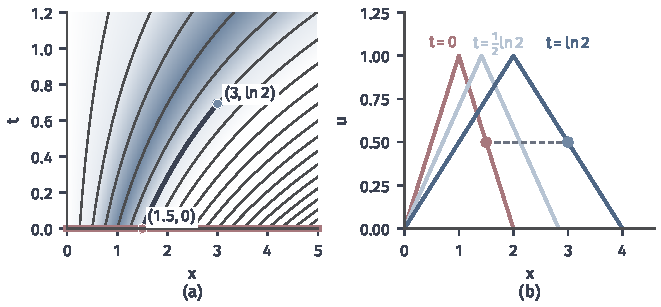
\includegraphics[width=112mm]{figures/06-differential-equations/02-partial-differential-equations/matplotlib/transp-curved/figure.pdf}
  \caption{速度场$v=x$对初值~\eqref{eq:transp-tent}的搬运。(a)特征线$x=x_0\mathrm{e}^{t}$（深灰）和解的时空热图，粗线把$(1.5,0)$（红）连到$(3,\ln2)$（蓝）。(b)初值（红）和$t=\frac12\ln2$、$t=\ln2$的解（蓝色由浅到深），虚线连接同一粒子的前后位置，高度不变。}
  \label{fig:transp-curved}
\end{BookInlineFigure}

速度场显含时间时做法相同，只是特征线的形状要由时间来决定。取$v=\cos t$，特征线$x=x_0+\sin t$来回摆动，解为$u_0(x-\sin t)$。取$v=xt$，特征线是$x=x_0\mathrm{e}^{t^{2}/2}$，解为$u_0(x\mathrm{e}^{-t^{2}/2})$。

图~\ref{fig:transp-timedep}展示了这两种情形。(a)中，每个时刻的速度在空间上处处相同，整个分布作为刚体来回移动。(b)中拉伸的速率随时间增大，特征线弯得越来越厉害。

\begin{BookInlineFigure}
  \centering
  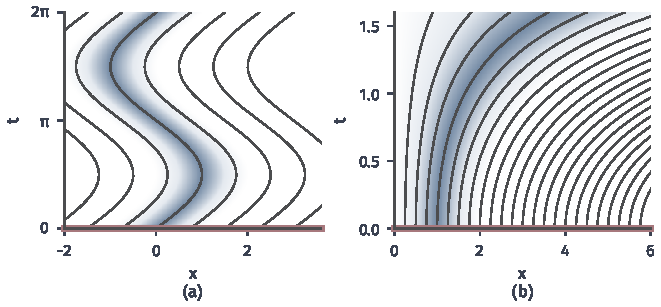
\includegraphics[width=112mm]{figures/06-differential-equations/02-partial-differential-equations/matplotlib/transp-timedep/figure.pdf}
  \caption{显含时间的速度场。深灰线是特征线，蓝色越深值越大，红线是初始线。(a)$v=\cos t$，初值是以$0$为中心、半宽为$1$的三角形。(b)$v=xt$，初值是式~\eqref{eq:transp-tent}。}
  \label{fig:transp-timedep}
\end{BookInlineFigure}

\paragraph{带源项的输运}
有源项时，由式~\eqref{eq:transp-along}，沿特征线的方程变成
\[
  \frac{\mathrm{d}}{\mathrm{d}t}u\bigl(\bm{x}(t),t\bigr)=f\bigl(\bm{x}(t),t\bigr).
\]
右端是沿已知曲线的已知函数，积分即得
\begin{equation}
  u\bigl(\bm{x}(t),t\bigr)=u_0(\bm{x}_0)+\int_0^{t}f\bigl(\bm{x}(s),s\bigr)\,\mathrm{d}s.
  \label{eq:transp-source-along}
\end{equation}
这就是图~\ref{fig:transp-trace}(c)的准确含义：$f$沿轨迹累积到$u$上。

\begin{example}[带源项的计算]
\label{ex:transp-source}
仍取$v=x$与初值~\eqref{eq:transp-tent}，源项取$f(x,t)=x$。沿特征线$x(s)=x_0\mathrm{e}^{s}$，由式~\eqref{eq:transp-source-along}，
\[
  u\bigl(x_0\mathrm{e}^{t},t\bigr)=u_0(x_0)+\int_0^{t}x_0\mathrm{e}^{s}\,\mathrm{d}s=u_0(x_0)+x_0\bigl(\mathrm{e}^{t}-1\bigr).
\]

把$x_0=x\mathrm{e}^{-t}$代回，得到
\[
  u(x,t)=u_0\bigl(x\mathrm{e}^{-t}\bigr)+x\bigl(1-\mathrm{e}^{-t}\bigr).
\]

计算点$(2,\ln2)$。它的出发位置是$x_0=1$，所以
\[
  u(2,\ln2)=u_0(1)+2\cdot\tfrac12=2.
\]
不计源项时，这一点的值是$1$，源项沿特征线累积的贡献是$1$。
\end{example}

图~\ref{fig:transp-source}(b)就是这个累积过程：沿出发于$x_0=1$的特征线，$u$从$1$增长到$\mathrm{e}^{t}$，浅蓝色的面积对应$\int_0^{t}\mathrm{e}^{s}\,\mathrm{d}s$。

\begin{BookInlineFigure}
  \centering
  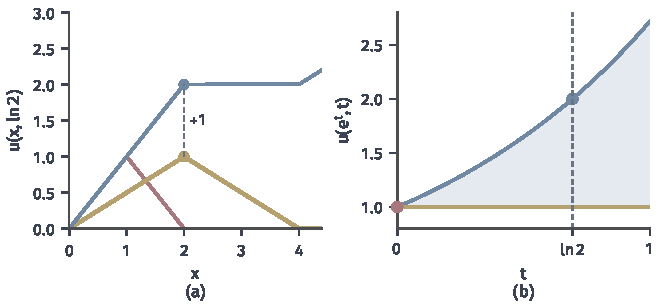
\includegraphics[width=112mm]{figures/06-differential-equations/02-partial-differential-equations/matplotlib/transp-source/figure.pdf}
  \caption{$v=x$、$f=x$的输运。(a)初值（红）、无源解（黄）和有源解（蓝）在$t=\ln2$的剖面，点$x=2$处两解相差$1$。(b)沿特征线$x=\mathrm{e}^{t}$的场值（蓝）与无源时的常值（黄），浅蓝区域是源项的累积，红点是初值。}
  \label{fig:transp-source}
\end{BookInlineFigure}

场的值也可以影响沿途的变化，典型的例子是线性衰减$f=-c(\bm{x},t)\,u+\tilde{f}$。此时沿特征线仍是一个常微分方程，只是变成了线性方程，用积分因子解出：
\begin{equation}
  u\bigl(\bm{x}(t),t\bigr)=\mathrm{e}^{-\int_0^{t}c\,\mathrm{d}r}\,u_0(\bm{x}_0)
  +\int_0^{t}\mathrm{e}^{-\int_s^{t}c\,\mathrm{d}r}\,\tilde{f}\bigl(\bm{x}(s),s\bigr)\,\mathrm{d}s,
  \label{eq:transp-reaction}
\end{equation}
其中$c$沿同一条特征线取值。例如$v=x$，$c=1$，$\tilde{f}=0$时，解为$u=\mathrm{e}^{-t}u_0(x\mathrm{e}^{-t})$。

\paragraph{与经典解的关系}
上面的计算默认了解存在且足够光滑，然后沿特征线推出它的值。这个过程反过来是否成立？按特征线公式造出的函数，是否真的满足方程？这需要速度场和数据的正则性。本章其余部分经常用到下面的条件，这里集中写出。

\medskip
\noindent\textbf{条件（V）.} $\bm{v}:\mathbb{R}^{d}\times[0,T]\to\mathbb{R}^{d}$连续，关于$\bm{x}$连续可微，Jacobian矩阵$\nabla\bm{v}$连续，且存在$L$，使对所有$(\bm{x},t)$有$\lVert\nabla\bm{v}(\bm{x},t)\rVert_2\leq L$。
\medskip

条件（V）说明$\bm{v}$关于$\bm{x}$全局Lipschitz，由第~\ref{chap:ode-existence-continuation}章的整体存在唯一性结论，方程~\eqref{eq:transp-char}过每一点$(\bm{x},t)$恰有一条定义在$[0,T]$上的解，记它在时刻$s$的位置为$\bm{X}(s;\bm{x},t)$。这条解由$\bm{X}(t;\bm{x},t)=\bm{x}$确定。

\begin{theorem}[特征线解与经典解]
\label{thm:transp-classical}
设$\bm{v}$满足条件（V），$u_0\in C^{1}(\mathbb{R}^{d})$，$f$在$\mathbb{R}^{d}\times[0,T]$上连续，关于$\bm{x}$连续可微且$\nabla f$连续。则输运问题~\eqref{eq:transp-ibvp}（$\Omega=\mathbb{R}^{d}$）有唯一的$C^{1}$解，
\begin{equation}
  u(\bm{x},t)=u_0\bigl(\bm{X}(0;\bm{x},t)\bigr)+\int_0^{t}f\bigl(\bm{X}(s;\bm{x},t),s\bigr)\,\mathrm{d}s.
  \label{eq:transp-char-solution}
\end{equation}
\end{theorem}

\begin{proof}
先证唯一性。设$u$是$C^{1}$解。沿过$(\bm{x},t)$的特征线，由式~\eqref{eq:transp-along}和方程，$u$的变化率等于$f$。从$0$到$t$积分，就得到式~\eqref{eq:transp-char-solution}，所以解只能是这个函数。

再证存在性，分两步：先说明这个函数是$C^{1}$的，再验证方程。令
\[
  \bm{\Psi}(\bm{x}_0,t)=\bigl(\bm{X}(t;\bm{x}_0,0),\,t\bigr).
\]
由解对初值的可微性（第~\ref{chap:ode-sensitivity}章），并结合$\partial_t\bm{X}=\bm{v}$，$\bm{\Psi}$是$C^{1}$映射。它的Jacobian矩阵是分块上三角的，对角块分别是$\mathrm{D}_{\bm{x}_0}\bm{X}$和$1$，行列式等于$\det\mathrm{D}_{\bm{x}_0}\bm{X}$，由第~\ref{chap:ode-sensitivity}章的Liouville公式知它恒正。

轨迹唯一性说明$\bm{\Psi}$是$\mathbb{R}^{d}\times[0,T]$到自身的双射。由反函数定理，$\bm{\Psi}^{-1}$也是$C^{1}$的，在$t=0,T$处按单侧导数理解。定义
\[
  W(\bm{x}_0,t)=u_0(\bm{x}_0)+\int_0^{t}f\bigl(\bm{X}(s;\bm{x}_0,0),s\bigr)\,\mathrm{d}s.
\]

$f$关于$\bm{x}$连续可微，所以$W$关于$\bm{x}_0$可以在积分号下求导，并且偏导数连续。$W$关于$t$的偏导数等于被积函数在$s=t$的值，也连续。所以$W\in C^{1}$，从而$u=W\circ\bm{\Psi}^{-1}\in C^{1}$。由于$\bm{X}(s;\bm{x}_0,0)=\bm{X}(s;\bm{x},t)$（同一条特征线），$u$就是式~\eqref{eq:transp-char-solution}的函数。

最后验证方程。由定义，$u(\bm{X}(t;\bm{x}_0,0),t)=W(\bm{x}_0,t)$。对$t$求导，并用式~\eqref{eq:transp-along}，
\[
  \bigl(\partial_tu+\bm{v}\cdot\nabla u\bigr)\bigl(\bm{X}(t;\bm{x}_0,0),t\bigr)=f\bigl(\bm{X}(t;\bm{x}_0,0),t\bigr).
\]
$\bm{\Psi}$是满射，所以方程在每一点成立。$t=0$时，$\bm{X}(0;\bm{x},0)=\bm{x}$，积分为零，初值条件成立。
\end{proof}

条件的作用可以逐一核对。$\bm{v}$的Lipschitz性保证过每点恰有一条特征线，否则“退回到$t=0$”的位置不确定，第~\ref{sec:transp-flow}节会给出具体的反例。$\nabla\bm{v}$的连续性让特征线关于初值$C^{1}$，这是解可微的来源。

$u_0$的$C^{1}$要求不能去掉。例~\ref{ex:transp-stretch}的三角形初值在$x=0,1,2$有折角，公式给出的解沿相应的三条特征线也有折角，它只在这些线之外是经典解。这说明特征线公式可以比方程本身走得更远，第~\ref{sec:transp-weak}节用测试函数解释这种解。有界区域的情形要把积分的下限换成特征线离开区域的时刻，并要求初值和入流数据在角点上按第~\ref{sec:transp-problem}节的方式衔接。

\section{流映射}
\label{sec:transp-flow}

上一节一次只跟踪一条特征线。把所有特征线放在一起看，固定两个时刻，每个粒子从前一时刻的位置走到后一时刻的位置，这就是一个空间到自身的映射。第~\ref{chap:ode-sensitivity}章已经研究过它，这里把要用的结论写下来。

\paragraph{流映射回顾}
对速度场$\bm{v}$，流映射$\bm{\varphi}_{s,t}(\bm{x})$表示时刻$s$位于$\bm{x}$的粒子在时刻$t$的位置，即
\begin{equation}
  \partial_t\bm{\varphi}_{s,t}(\bm{x})=\bm{v}\bigl(\bm{\varphi}_{s,t}(\bm{x}),t\bigr),\qquad
  \bm{\varphi}_{s,s}(\bm{x})=\bm{x}.
  \label{eq:transp-flow}
\end{equation}
上一节的$\bm{X}(s;\bm{x},t)$就是$\bm{\varphi}_{t,s}(\bm{x})$。

在条件（V）下，$\bm{\varphi}_{s,t}$是$\mathbb{R}^{d}$到自身的$C^{1}$双射。第~\ref{chap:ode-sensitivity}章还给出了两条代数规则：走两段等于走一段，走过去再走回来回到原处，即
\begin{equation}
  \bm{\varphi}_{r,t}\circ\bm{\varphi}_{s,r}=\bm{\varphi}_{s,t},\qquad
  \bm{\varphi}_{t,s}=\bm{\varphi}_{s,t}^{-1}.
  \label{eq:transp-flow-rules}
\end{equation}

\paragraph{输运解的表示}
用流映射重写式~\eqref{eq:transp-char-solution}，得到
\begin{equation}
  u(\cdot,t)=u_0\circ\bm{\varphi}_{t,0}+\int_0^{t}f(\cdot,s)\circ\bm{\varphi}_{t,s}\,\mathrm{d}s.
  \label{eq:transp-flow-solution}
\end{equation}
这里出现的是逆向的映射$\bm{\varphi}_{t,0}$。粒子带着值$u_0(\bm{x}_0)$从$\bm{x}_0$走到$\bm{\varphi}_{0,t}(\bm{x}_0)$，要想知道固定位置$\bm{y}$的值，必须先问“现在位于$\bm{y}$的粒子原来在哪里”，然后到初值里去查。

图~\ref{fig:transp-lookup}把例~\ref{ex:transp-stretch}的三个粒子连了起来。这时$\varphi_{0,\ln2}(x)=2x$，上下两条曲线上用箭头相连的点高度相同。要读下面的曲线在$y=3$处的值，就从$y=3$沿箭头退回$x_0=1.5$，到上面的曲线上读出$0.5$。

\begin{BookInlineFigure}
  \centering
  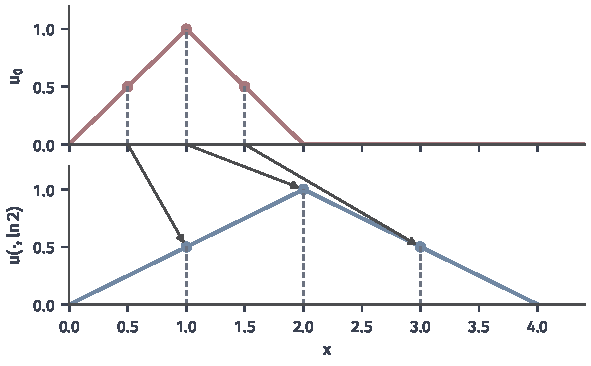
\includegraphics[width=100mm]{figures/06-differential-equations/02-partial-differential-equations/matplotlib/transp-lookup/figure.pdf}
  \caption{用流映射搬运场值，$v=x$，$t=\ln2$。上图是初值（红），下图是搬运后的解（蓝）。箭头把位置$x_0=0.5,1,1.5$连到$2x_0$，点的高度保持不变。}
  \label{fig:transp-lookup}
\end{BookInlineFigure}

同一个解有两种描述方式。跟着粒子看，$u(\bm{\varphi}_{0,t}(\bm{x}_0),t)=u_0(\bm{x}_0)$，这称为\term{Lagrange描述}（Lagrangian description），标号是粒子的初始位置。站在固定位置看，$u(\bm{y},t)=u_0(\bm{\varphi}_{t,0}(\bm{y}))$，这称为\term{Euler描述}（Eulerian description），标号是当前位置。两者用流映射互相转换，这也是公式中需要逆映射的原因。

$v=x$时流映射是$\varphi_{s,t}(x)=x\mathrm{e}^{t-s}$。规则~\eqref{eq:transp-flow-rules}在这里就是指数的相加。$v=xt$时流映射依赖两个时刻：
\[
  \varphi_{s,t}(x)=x\exp\Bigl(\frac{t^{2}-s^{2}}{2}\Bigr).
\]
这时$\varphi_{0,1}$的倍数是$\mathrm{e}^{1/2}$，$\varphi_{1,2}$的倍数是$\mathrm{e}^{3/2}$，相乘得到$\varphi_{0,2}$的倍数$\mathrm{e}^{2}$，符合式~\eqref{eq:transp-flow-rules}；但第二段时间的倍数不等于第一段，同样长的时间间隔走出的倍数不同，所以必须记住起止两个时刻。

平面上的情形类似。旋转场$\bm{v}=(-x_2,x_1)^{\top}$的流映射是旋转矩阵，鞍点场$\bm{v}=(x_1,-x_2)^{\top}$沿一个方向拉伸，沿另一个方向压缩：
\[
  \bm{\varphi}_{t}^{\mathrm{rot}}(\bm{x})=
  \begin{pmatrix}\cos t&-\sin t\\ \sin t&\cos t\end{pmatrix}\bm{x},\qquad
  \bm{\varphi}_{t}^{\mathrm{sad}}(\bm{x})=
  \begin{pmatrix}\mathrm{e}^{t}&0\\ 0&\mathrm{e}^{-t}\end{pmatrix}\bm{x}.
\]

图~\ref{fig:transp-2d-advect}用式~\eqref{eq:transp-flow-solution}搬运了一个由两团组成的初值。旋转把它转了四分之一圈，形状不变；鞍点流把它在一个方向拉长、另一个方向压扁。两种情形下，解的最大值都和初值相同，因为$u$只是被搬动，没有哪个粒子携带的值发生了变化。

\begin{BookInlineFigure}
  \centering
  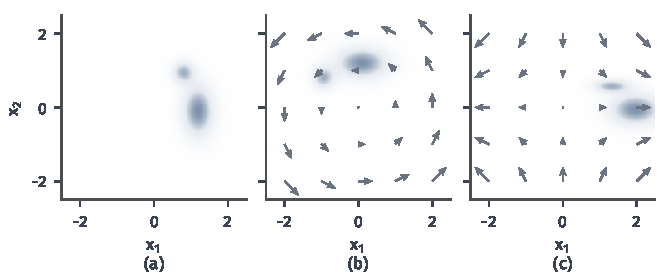
\includegraphics[width=112mm]{figures/06-differential-equations/02-partial-differential-equations/matplotlib/transp-2d-advect/figure.pdf}
  \caption{平面上的搬运，蓝色越深值越大，三幅图共用一个色阶，灰色箭头是速度场的方向。(a)初值。(b)旋转场，$t=\pi/2$。(c)鞍点场$\bm{v}=(x_1,-x_2)^{\top}$，$t=0.5$。}
  \label{fig:transp-2d-advect}
\end{BookInlineFigure}

\paragraph{逆映射的范围}
条件（V）保证了粒子不会在有限时间内跑到无穷远，也就保证了$\bm{\varphi}_{s,t}$在全空间上定义。去掉全局Lipschitz条件后，轨迹可能爆炸，逆映射的定义域就受到限制。

取$v=x^{2}$，第~\ref{chap:ode-sensitivity}章已经算出它的流映射：
\[
  \varphi_{0,t}(x)=\frac{x}{1-tx},\qquad x<\frac1t\quad(t>0).
\]
当$x$跑遍$(-\infty,1/t)$时，$\varphi_{0,t}(x)$跑遍$(-1/t,\infty)$。于是从初始线出发的粒子在时刻$t$只占据$y>-1/t$，反解得到的逆映射只在这个范围内有定义：
\[
  \varphi_{t,0}(y)=\frac{y}{1+ty},\qquad y>-\frac1t.
\]

图~\ref{fig:transp-flow-domain}(a)中，浅红色区域$\{x\leq-1/t\}$里的点没有来自初始线的特征线，它们的值由初值无法确定，这些特征线要追溯到“从$-\infty$进来”。另一方面，$x_0\geq1/t$的粒子在时刻$t$之前已经跑到了$+\infty$。例如$(y,t)=(1,1)$的出发位置是$1/2$，而$(y,t)=(-2,1)$没有出发位置。

\begin{BookInlineFigure}
  \centering
  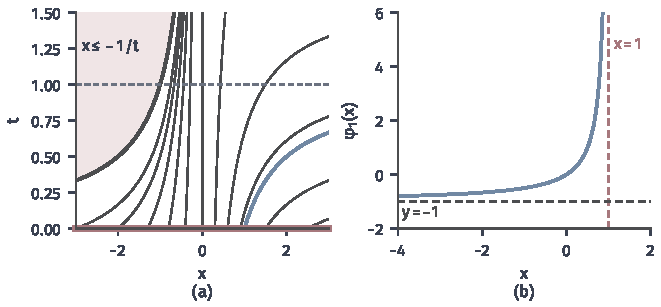
\includegraphics[width=112mm]{figures/06-differential-equations/02-partial-differential-equations/matplotlib/transp-flow-domain/figure.pdf}
  \caption{速度场$v=x^{2}$的流映射只在部分区域可逆。(a)特征线（深灰），蓝线是从$x_0=1$出发、在$t=1$爆炸的轨迹，粗深灰线$x=-1/t$是从初始线可达区域的边界，浅红区域无法追溯到初始线。(b)$\varphi_{0,1}(x)=x/(1-x)$，定义在$x<1$，值域是$(-1,\infty)$。}
  \label{fig:transp-flow-domain}
\end{BookInlineFigure}

所以一般情形下，式~\eqref{eq:transp-flow-solution}只在点$(\bm{y},t)$的反向轨迹能够回到$t=0$时才有意义。这时解存在的区域是流映射的值域，而不是整个时空。

\paragraph{轨迹唯一性}
即使轨迹全局存在，失去唯一性也会破坏这种表示。取$v(x)=2\sqrt{\lvert x\rvert}$，它在$x=0$处不Lipschitz。从负轴出发的粒子向右运动，在有限时间到达$0$，然后可以在$0$停留任意一段时间，再离开。过$(0,c)$向右离开的轨迹是$x=(t-c)^{2}$。

看图~\ref{fig:transp-nonunique}(a)中的点$P=(1,2)$。反向追踪得到$x=(r-1)^{2}$，在$r=1$到达$0$。再往回，有多条轨迹都能走到$(0,1)$：可以一直停在$0$，也可以来自负轴。凡是出发位置$x_0\in[-1,0]$的粒子，都可能在时刻$2$到达$P$，图中用红色粗线标出这些出发位置，黄色虚线是其中两条。

如果$u$是$C^{1}$解，它沿每条这样的轨迹都不变，所以$u_0$在$[-1,0]$上必须是常数。只要初值在这一段上不是常数，方程就没有$C^{1}$解。

\begin{BookInlineFigure}
  \centering
  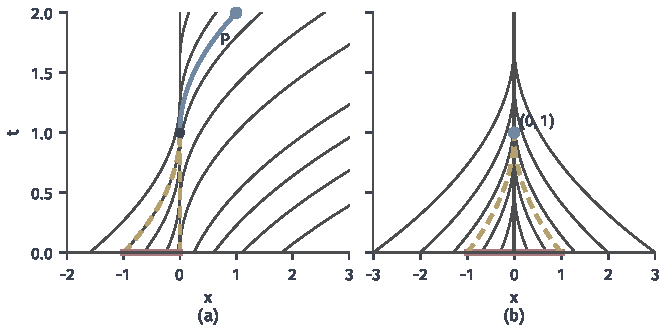
\includegraphics[width=112mm]{figures/06-differential-equations/02-partial-differential-equations/matplotlib/transp-nonunique/figure.pdf}
  \caption{速度场不Lipschitz时的轨迹。(a)$v=2\sqrt{\lvert x\rvert}$，轨迹在$x=0$处分叉，蓝线是到达$P$的最后一段，黄色虚线是到达$(0,1)$的两条路径，红色粗线是可能的出发位置$[-1,0]$。(b)$v=-2\,\mathrm{sgn}(x)\sqrt{\lvert x\rvert}$，轨迹并入$x=0$，从蓝点反向追踪的出发位置是红色粗线$[-1,1]$。}
  \label{fig:transp-nonunique}
\end{BookInlineFigure}

图~\ref{fig:transp-nonunique}(b)是反方向的情形。$v=-2\,\mathrm{sgn}(x)\sqrt{\lvert x\rvert}$下，粒子都流向$0$，正向轨迹是唯一的，但$[-1,1]$中的粒子在$t=1$时都已并入$0$，$\varphi_{0,1}$不是单射，逆映射不存在。从$(0,1)$反向追踪得到一整段出发位置，$u_0$在$[-1,1]$上不是常数时，同样不存在$C^{1}$解。

这两个例子说明，输运解的表示依赖于$\bm{\varphi}_{s,t}$的可逆性，可逆性又依赖轨迹在正反两个方向上的唯一性。以下都假设条件（V），需要讨论局部情形时，会明确说明定义域。


\section{连续性方程}
\label{sec:transp-continuity}

回到例~\ref{ex:transp-stretch}。三角形被$v=x$搬运到$t=\ln2$时，底变成了原来的两倍，高度不变，曲线下的面积从$1$变成了$2$。如果$u$表示粒子携带的标签，这没有问题；如果用它表示单位长度的墨水质量，总质量就凭空翻了一倍。质量不会凭空产生，所以墨水的浓度不满足输运方程，我们需要一个由质量平衡出发的新方程。

\paragraph{一维的质量平衡}
用$\rho(x,t)$表示单位长度的质量，取一段固定的区间$[a,b]$。流量$\rho v$是单位时间穿过某一点的质量，正号表示向右。如图~\ref{fig:transp-balance}(a)，区间内质量的变化等于从$a$流入的减去从$b$流出的，再加上区间内的源项$f$：
\[
  \frac{\mathrm{d}}{\mathrm{d}t}\int_a^{b}\rho\,\mathrm{d}x
  =\rho v\big|_{x=a}-\rho v\big|_{x=b}+\int_a^{b}f\,\mathrm{d}x.
\]

设$\rho$、$v$足够光滑，用微积分基本定理把两端的差写成积分：
\[
  \int_a^{b}\bigl(\partial_t\rho+\partial_x(\rho v)-f\bigr)\,\mathrm{d}x=0.
\]
区间是任取的，被积函数连续，所以它恒为零，这就是一维的连续性方程。

\begin{BookInlineFigure}
  \centering
  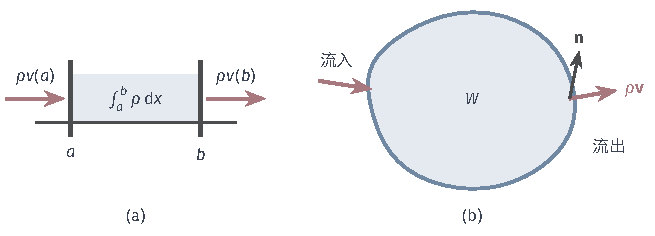
\includegraphics[width=111mm]{figures/06-differential-equations/02-partial-differential-equations/tikz/transp-balance/figure.pdf}
  \caption{控制区域的质量平衡。(a)区间$[a,b]$内的质量变化由两端的流量差决定。(b)平面区域$W$，红色箭头是质量流$\rho\bm{v}$，它在外法向$\bm{n}$上的投影为正时流出、为负时流入。}
  \label{fig:transp-balance}
\end{BookInlineFigure}

\paragraph{多维的质量平衡}
取固定的\term{控制区域}（control region）$W\subset\mathbb{R}^{d}$，如图~\ref{fig:transp-balance}(b)，边界光滑。穿过边界的质量流是$\rho\bm{v}\cdot\bm{n}$，于是
\begin{equation}
  \frac{\mathrm{d}}{\mathrm{d}t}\int_W\rho\,\mathrm{d}\bm{x}
  =-\int_{\partial W}\rho\bm{v}\cdot\bm{n}\,\mathrm{d}S+\int_Wf\,\mathrm{d}\bm{x}.
  \label{eq:transp-balance}
\end{equation}
由散度定理（见\BookChapterRef{chap:integral-theorems}{卷二第27章“积分定理”}），边界积分等于$\int_W\nabla\cdot(\rho\bm{v})\,\mathrm{d}\bm{x}$。由$W$的任意性，得到下面的方程。

\begin{definition}[连续性方程]
\label{def:transp-continuity}
给定速度场$\bm{v}$和源项$f$，未知密度$\rho(\bm{x},t)$满足的方程
\begin{equation}
  \partial_t\rho+\nabla\cdot(\rho\bm{v})=f
  \label{eq:transp-continuity}
\end{equation}
称为\term{连续性方程}（continuity equation）。
\end{definition}

把散度展开，可以看清它与输运方程的差别：
\begin{equation}
  \partial_t\rho+\bm{v}\cdot\nabla\rho=f-\rho\,\nabla\cdot\bm{v}.
  \label{eq:transp-divergence-correction}
\end{equation}
左端仍然是物质导数，右端多了一项$-\rho\nabla\cdot\bm{v}$，它就是散度修正。粒子携带的值不变，但$\rho$是“粒子周围的拥挤程度”，流动把周围的空间撑大或压小，这个量就要变。

当$\nabla\cdot\bm{v}=0$时修正项消失，两个方程完全一样，这样的速度场称为\term{无散度速度场}（divergence-free velocity field）。一般的速度场下两个方程不同，同一个初值走出的结果也不同。

\begin{example}[同一流动下的值与密度]
\label{ex:transp-rho-stretch}
仍取$v=x$，初值同式~\eqref{eq:transp-tent}。连续性方程是式~\eqref{eq:transp-reaction}的$c=\nabla\cdot v=1$情形，沿特征线的解是
\[
  \rho(x,t)=\mathrm{e}^{-t}\rho_0\bigl(x\mathrm{e}^{-t}\bigr).
\]

直接代入验证。对$t$求偏导，
\[
  \partial_t\rho=-\mathrm{e}^{-t}\rho_0-x\mathrm{e}^{-2t}\rho_0'.
\]
$\partial_x(x\rho)=\rho+x\partial_x\rho$，其中第一项是$\mathrm{e}^{-t}\rho_0$，第二项是$x\mathrm{e}^{-2t}\rho_0'$。两式相加为零。

点$(3,\ln2)$的出发位置是$1.5$。输运方程的解是$u(3,\ln2)=0.5$，连续性方程的解是
\[
  \rho(3,\ln2)=\tfrac12\cdot\rho_0(1.5)=0.25.
\]

积分验证总量。三角形的面积是$1$，时刻$t$时，对$\rho$换元$z=x\mathrm{e}^{-t}$，
\[
  \int_{\mathbb{R}}\rho(x,t)\,\mathrm{d}x=\int_{\mathbb{R}}\rho_0(z)\,\mathrm{d}z=1.
\]
同样的换元用在$u$上，多出的因子$\mathrm{e}^{t}$没有抵消，于是$\int u(x,t)\,\mathrm{d}x=\mathrm{e}^{t}$。
\end{example}

图~\ref{fig:transp-value-density}把这个例子放在一起比较。(a)和(b)的初值、流动完全相同，(a)中三角形的高度不变，面积翻倍；(b)中高度减半，面积不变。(c)是沿$x_0=1$这条特征线的三个量：$u$恒为$1$，体积倍率$J=\mathrm{e}^{t}$增长，密度$\rho=\mathrm{e}^{-t}$下降，乘积$\rho J$恒为$1$。

\begin{BookInlineFigure}
  \centering
  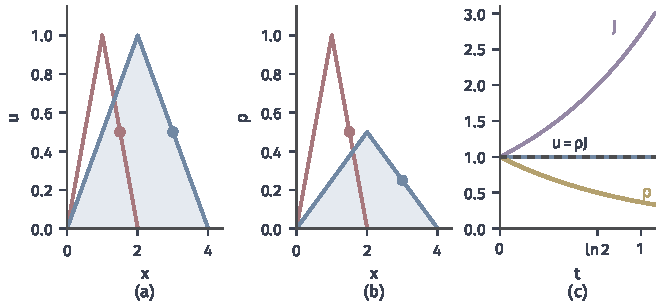
\includegraphics[width=112mm]{figures/06-differential-equations/02-partial-differential-equations/matplotlib/transp-value-density/figure.pdf}
  \caption{$v=x$，$t=\ln2$，初值同式~\eqref{eq:transp-tent}（红）。(a)场值$u$，浅蓝面积为$2$。(b)密度$\rho$，浅蓝面积为$1$，两图中的点都是$x_0=1.5$及其像。(c)沿$x_0=1$的特征线：$u$（蓝）、$\rho$（黄）、体积倍率$J$（紫）与乘积$\rho J$（虚线）。}
  \label{fig:transp-value-density}
\end{BookInlineFigure}

这里有两件容易混淆的事。沿轨迹密度不变，说的是物质导数为零，这只在$\nabla\cdot\bm{v}=0$时成立；总质量不变，说的是全空间的积分不随时间变化，它在$\bm{v}$不是无散度时同样成立，只要密度衰减足够快、没有质量从边界流失。例~\ref{ex:transp-rho-stretch}中总质量不变，沿轨迹的密度却在下降。

\subsection{体积变化}
\label{sec:transp-volume}

修正项$\rho\nabla\cdot\bm{v}$的来历，要从体积的变化说起。想象一维流动中相邻的两个粒子，相距$\Delta x$。前面的粒子比后面的多走了$\bigl(v(x+\Delta x)-v(x)\bigr)\,\mathrm{d}t$，所以它们的间距以$\partial_xv\,\Delta x$的速度增大，相对增长率就是$\partial_xv$。散度是这个现象在多维的写法。

\paragraph{Jacobian的演化}
记流映射的Jacobian行列式
\begin{equation}
  J_{s,t}(\bm{x})=\det\mathrm{D}\bm{\varphi}_{s,t}(\bm{x}).
  \label{eq:transp-jacobian}
\end{equation}

第~\ref{chap:ode-sensitivity}章证明了，Jacobian矩阵沿轨迹满足线性方程
\[
  \partial_t\mathrm{D}\bm{\varphi}_{s,t}=\nabla\bm{v}\bigl(\bm{\varphi}_{s,t},t\bigr)\,\mathrm{D}\bm{\varphi}_{s,t}.
\]
它的行列式满足Liouville公式，在这里的记号下，这个公式是
\begin{equation}
  \partial_tJ_{s,t}=\bigl(\nabla\cdot\bm{v}\bigr)\bigl(\bm{\varphi}_{s,t},t\bigr)\,J_{s,t},\qquad J_{s,s}=1,
  \label{eq:transp-liouville}
\end{equation}
解出来就是
\begin{equation}
  J_{s,t}(\bm{x})=\exp\int_s^{t}\bigl(\nabla\cdot\bm{v}\bigr)\bigl(\bm{\varphi}_{s,r}(\bm{x}),r\bigr)\,\mathrm{d}r>0.
  \label{eq:transp-liouville-solution}
\end{equation}

结合换元公式，可测集$\bm{W}$被搬运后的体积是$\int_{\bm{W}}J_{s,t}\,\mathrm{d}\bm{x}$。这说明$J_{s,t}$是局部的体积倍率，散度是体积倍率在瞬时的对数变化率。

\begin{example}[Logistic速度场的体积倍率]
\label{ex:transp-logistic-jacobian}
取$\Omega=(0,1)$，$v(x)=x(1-x)$，它正是第~\ref{chap:ode-sensitivity}章用过的Logistic方程的右端。流映射是
\[
  \varphi_{t}(x)=\frac{x\mathrm{e}^{t}}{1-x+x\mathrm{e}^{t}}.
\]
对$x$求导，
\[
  J_{0,t}(x)=\partial_x\varphi_{t}(x)=\frac{\mathrm{e}^{t}}{\bigl(1-x+x\mathrm{e}^{t}\bigr)^{2}}.
\]

$t=\ln2$时，$J_{0,\ln2}(x)=2/(1+x)^{2}$。取$x=1/3$，得到
\[
  J_{0,\ln2}(1/3)=\frac{2}{(4/3)^{2}}=\frac98.
\]

用式~\eqref{eq:transp-liouville-solution}核对。这条轨迹是$\varphi_s(1/3)=\mathrm{e}^{s}/(2+\mathrm{e}^{s})$，散度沿它取值$1-2\varphi_s$，积分得
\[
  \int_0^{\ln2}\Bigl(1-\frac{2\mathrm{e}^{s}}{2+\mathrm{e}^{s}}\Bigr)\mathrm{d}s
  =\ln2-2\ln\frac43=\ln\frac98.
\]
指数正好是$9/8$，与直接求导相同。
\end{example}

图~\ref{fig:transp-spreading}(a)从$[0,1]$上等间距的点出发画特征线。左半部分的线逐渐拉开，右半部分的线向$x=1$挤压，线的疏密直接反映出体积倍率。(b)是$t=\ln2$时的倍率$J_{0,\ln2}$：左边大于$1$，表示膨胀；右边小于$1$，表示压缩。绿点是用流映射的差分算出来的，与公式重合。

\begin{BookInlineFigure}
  \centering
  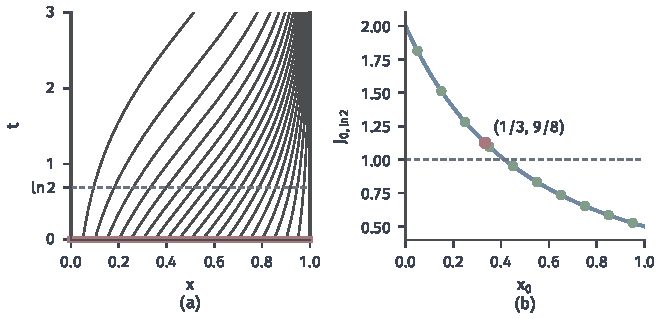
\includegraphics[width=112mm]{figures/06-differential-equations/02-partial-differential-equations/matplotlib/transp-spreading/figure.pdf}
  \caption{Logistic速度场$v=x(1-x)$。(a)从等间距的初始位置（红线）出发的特征线，两端的粗线是不动的边界。(b)$t=\ln2$的体积倍率（蓝），绿点是对流映射做中心差分的结果，红点是例~\ref{ex:transp-logistic-jacobian}的$(1/3,9/8)$，虚线是$J=1$。}
  \label{fig:transp-spreading}
\end{BookInlineFigure}

$\nabla\cdot\bm{v}\equiv0$时，由式~\eqref{eq:transp-liouville-solution}，$J_{s,t}\equiv1$，流映射保持体积。这是第~\ref{sec:transp-flow}节旋转场和鞍点场的共同之处。图~\ref{fig:transp-volume-flows}比较了三种平面流。

旋转场的散度是$\partial_1(-x_2)+\partial_2x_1=0$，鞍点场是$1-1=0$，面积都不变。放大场$\bm{v}=(x_1,x_2)^{\top}$的散度是$2$，$J=\mathrm{e}^{2t}$，$t=\ln2$时面积放大到$4$倍，$0.25$变成了$1$。一般的流要保留这个倍率，不能当作$1$。

\begin{BookInlineFigure}
  \centering
  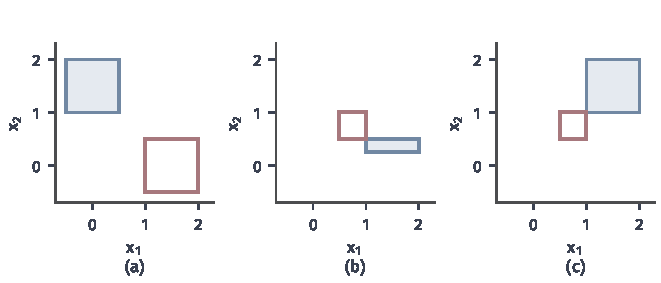
\includegraphics[width=112mm]{figures/06-differential-equations/02-partial-differential-equations/matplotlib/transp-volume-flows/figure.pdf}
  \caption{正方形（红框）被流映射搬运后的像（浅蓝）。(a)旋转场，$t=\pi/2$，面积$1$不变。(b)鞍点场，$t=\ln2$，正方形变成长方形，面积仍为$0.25$。(c)放大场，$t=\ln2$，面积由$0.25$变为$1$。}
  \label{fig:transp-volume-flows}
\end{BookInlineFigure}

\subsection{密度搬运}
\label{sec:transp-density}

有了体积倍率，可以直接算出密度。如图~\ref{fig:transp-pushforward}，一小块区域$\bm{W}$里的质量是$m\approx\rho_0(\bm{x})\lvert\bm{W}\rvert$。流动把它带到$\bm{\varphi}_{0,t}(\bm{W})$，质量不变，体积乘上了$J_{0,t}(\bm{x})$，所以新的密度应当是$\rho_0(\bm{x})/J_{0,t}(\bm{x})$。

\begin{BookInlineFigure}
  \centering
  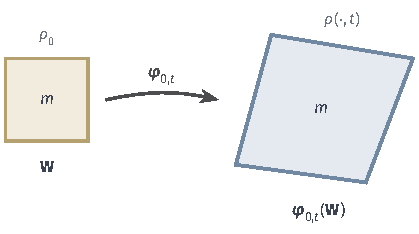
\includegraphics[width=70.9mm]{figures/06-differential-equations/02-partial-differential-equations/tikz/transp-pushforward/figure.pdf}
  \caption{一小块质量被流映射搬运。质量$m$不变，体积变为$J_{0,t}$倍，所以密度除以$J_{0,t}$。}
  \label{fig:transp-pushforward}
\end{BookInlineFigure}

\paragraph{推前测度}
这个想法用测度来说最干净。记初始质量分布为$\mu_0$，$\mathrm{d}\mu_0=\rho_0\,\mathrm{d}\bm{x}$。时刻$t$落在集合$B$中的质量，正好是初始时刻位于$\bm{\varphi}_{t,0}(B)$中的质量，于是
\begin{equation}
  \mu_t(B)=\mu_0\bigl(\bm{\varphi}_{t,0}(B)\bigr),\qquad
  \mu_t=(\bm{\varphi}_{0,t})_{\#}\mu_0.
  \label{eq:transp-pushforward-measure}
\end{equation}
也就是说，$\mu_t$是$\mu_0$在流映射下的推前测度，定义和基本性质见\BookChapterRef{chap:pushforward-measures}{卷四第9章“推前测度”}。

\begin{theorem}[密度搬运公式]
\label{thm:transp-density}
设$\bm{v}$满足条件（V），$\nabla\cdot\bm{v}$关于$\bm{x}$连续可微且偏导数连续，$\rho_0\in C^{1}(\mathbb{R}^{d})$。则方程~\eqref{eq:transp-continuity}（$f=0$）有唯一满足$\rho(\cdot,0)=\rho_0$的$C^{1}$解，它由下式确定：
\begin{equation}
  \rho\bigl(\bm{\varphi}_{0,t}(\bm{x}),t\bigr)\,J_{0,t}(\bm{x})=\rho_0(\bm{x}).
  \label{eq:transp-density}
\end{equation}
进而对任意非负可测函数$h$，有
\begin{equation}
  \int_{\mathbb{R}^{d}}\rho(\bm{y},t)\,h(\bm{y})\,\mathrm{d}\bm{y}
  =\int_{\mathbb{R}^{d}}\rho_0(\bm{x})\,h\bigl(\bm{\varphi}_{0,t}(\bm{x})\bigr)\,\mathrm{d}\bm{x}.
  \label{eq:transp-pushforward}
\end{equation}
若$\rho_0\geq0$，则$\rho\geq0$；取$h=1$，总质量不随时间变化。
\end{theorem}

\begin{proof}
设$\rho$是$C^{1}$解。沿轨迹，由式~\eqref{eq:transp-along}和式~\eqref{eq:transp-liouville}，
\[
  \frac{\mathrm{d}}{\mathrm{d}t}\Bigl[\rho\bigl(\bm{\varphi}_{0,t}(\bm{x}),t\bigr)J_{0,t}(\bm{x})\Bigr]
  =\bigl(\partial_t\rho+\bm{v}\cdot\nabla\rho+\rho\nabla\cdot\bm{v}\bigr)\bigl(\bm{\varphi}_{0,t}(\bm{x}),t\bigr)\,J_{0,t}(\bm{x}).
\]
括号里正是$\partial_t\rho+\nabla\cdot(\rho\bm{v})=0$，所以$\rho J$沿轨迹不变，取$t=0$的值即得式~\eqref{eq:transp-density}，唯一性得证。

反过来，令$R(\bm{x},t)=\rho_0(\bm{x})/J_{0,t}(\bm{x})$。$\nabla\cdot\bm{v}$关于$\bm{x}$是$C^{1}$的，由式~\eqref{eq:transp-liouville-solution}，$J_{0,t}$关于$(\bm{x},t)$是$C^{1}$的且恒正，$R$也是。沿定理~\ref{thm:transp-classical}证明中的映射$\bm{\Psi}$，定义$\rho=R\circ\bm{\Psi}^{-1}$，它是$C^{1}$的，并满足式~\eqref{eq:transp-density}。再用上面的等式把导数读出来，由$J_{0,t}>0$和$\bm{\Psi}$是满射，方程在每一点成立。

式~\eqref{eq:transp-pushforward}由换元$\bm{y}=\bm{\varphi}_{0,t}(\bm{x})$得到。换元产生因子$J_{0,t}$，由式~\eqref{eq:transp-density}，被积函数中$\rho J$恰好等于$\rho_0$：
\[
  \begin{aligned}
  \int\rho(\bm{y},t)h(\bm{y})\,\mathrm{d}\bm{y}
  &=\int\rho\bigl(\bm{\varphi}_{0,t}(\bm{x}),t\bigr)h\bigl(\bm{\varphi}_{0,t}(\bm{x})\bigr)J_{0,t}(\bm{x})\,\mathrm{d}\bm{x}\\
  &=\int\rho_0(\bm{x})h\bigl(\bm{\varphi}_{0,t}(\bm{x})\bigr)\,\mathrm{d}\bm{x}.
  \end{aligned}
\]
非负性由式~\eqref{eq:transp-density}和$J_{0,t}>0$得到。
\end{proof}

式~\eqref{eq:transp-density}是本章的核心：密度倍率$1/J$与体积倍率$J$逐点抵消，乘积沿轨迹不变。取$h$为集合$B$的指示函数，式~\eqref{eq:transp-pushforward}就是式~\eqref{eq:transp-pushforward-measure}。定理还要求$\nabla\cdot\bm{v}$对$\bm{x}$可微，这是为了得到$C^{1}$解；只求弱解时可以去掉，见第~\ref{sec:transp-weak}节。

有源项时，同样的计算给出$\frac{\mathrm{d}}{\mathrm{d}t}[\rho J]=fJ$，沿轨迹积分得到
\begin{equation}
  \rho\bigl(\bm{\varphi}_{0,t}(\bm{x}),t\bigr)\,J_{0,t}(\bm{x})
  =\rho_0(\bm{x})+\int_0^{t}f\bigl(\bm{\varphi}_{0,s}(\bm{x}),s\bigr)\,J_{0,s}(\bm{x})\,\mathrm{d}s.
  \label{eq:transp-density-source}
\end{equation}

\begin{example}[区间上的密度搬运]
\label{ex:transp-logistic-density}
在$(0,1)$上取$v=x(1-x)$，初始密度$\rho_0=1$。由例~\ref{ex:transp-logistic-jacobian}的结果，逆流映射是
\[
  \varphi_{t,0}(y)=\frac{y\mathrm{e}^{-t}}{1-y+y\mathrm{e}^{-t}}.
\]

把$J_{0,t}$用当前位置$y$表示。令$D=1-y+y\mathrm{e}^{-t}$，代入得$1-x+x\mathrm{e}^{t}=1/D$，于是$J_{0,t}=\mathrm{e}^{t}D^{2}$。由式~\eqref{eq:transp-density}，
\[
  \rho(y,t)=\frac{\mathrm{e}^{-t}}{\bigl(1-y+y\mathrm{e}^{-t}\bigr)^{2}}.
\]

取$t=\ln2$，$y=1/2$。出发位置是$x=\varphi_{\ln2,0}(1/2)=1/3$，倍率是$9/8$，所以
\[
  \rho(1/2,\ln2)=\frac{8}{9}.
\]
代入上面的公式核对：$D=3/4$，$\rho=\tfrac12\cdot\tfrac{16}{9}=\tfrac89$。

再验证总质量。$t=\ln2$时$\rho(y,\ln 2)=\tfrac12(1-y/2)^{-2}$，
\[
  \int_0^{1}\frac12\Bigl(1-\frac{y}{2}\Bigr)^{-2}\mathrm{d}y=\Bigl[\frac{1}{1-y/2}\Bigr]_0^{1}=2-1=1.
\]
\end{example}

图~\ref{fig:transp-logistic-density}(a)是这个密度在不同时刻的形状。均匀的初始分布逐渐向右端集中，绿色直方图是$40000$个按初始分布抽取的粒子在$t=\ln4$的位置，与公式吻合。

(b)从另一个角度看。质量$\int_0^{y}\rho\,\mathrm{d}x$等于初始时位于$(0,\varphi_{t,0}(y))$中的质量，而$\rho_0=1$，所以累积质量恰好是逆流映射本身。$t=\ln2$时，左半区间的质量是$\varphi_{\ln2,0}(1/2)=1/3$。

\begin{BookInlineFigure}
  \centering
  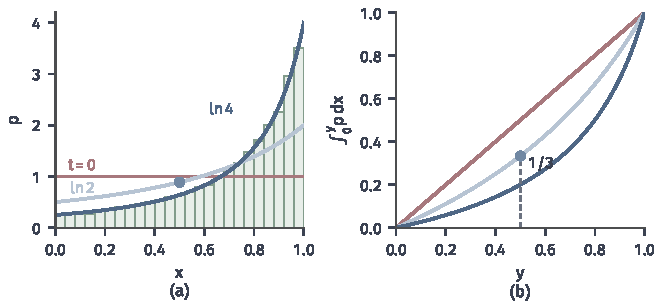
\includegraphics[width=112mm]{figures/06-differential-equations/02-partial-differential-equations/matplotlib/transp-logistic-density/figure.pdf}
  \caption{$(0,1)$上$v=x(1-x)$对均匀密度的搬运。(a)密度$\rho$：$t=0$（红）、$t=\ln2$与$t=\ln4$（蓝色由浅到深），绿色直方图是$40000$个粒子（固定种子）在$t=\ln4$的分布，蓝点是$(1/2,8/9)$。(b)累积质量，蓝点表示$t=\ln2$时左半区间的质量为$1/3$。}
  \label{fig:transp-logistic-density}
\end{BookInlineFigure}

平面上的情形相同。图~\ref{fig:transp-density-2d}把一个Gaussian形的密度分别交给三种流，运行时间都是$t=1$，初始峰值是$1$。放大场$\bm{v}=\bm{x}/2$的散度是$1$，峰值降到$\mathrm{e}^{-1}\approx0.37$；鞍点场$\bm{v}=(x_1/2,-x_2/2)^{\top}$的散度是$0$，形状变了，峰值不变；收缩场$\bm{v}=-\bm{x}/2$的散度是$-1$，峰值升到$\mathrm{e}\approx2.72$。

\begin{BookInlineFigure}
  \centering
  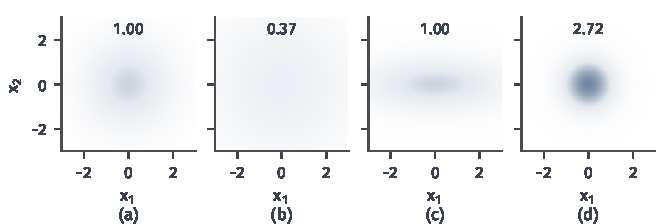
\includegraphics[width=112mm]{figures/06-differential-equations/02-partial-differential-equations/matplotlib/transp-density-2d/figure.pdf}
  \caption{同一Gaussian形密度的搬运，蓝色越深密度越大，图中数字是峰值。(a)初值。(b)放大场，$t=1$。(c)无散度的鞍点场，$t=1$。(d)收缩场，$t=1$。四幅图共用一个色阶。}
  \label{fig:transp-density-2d}
\end{BookInlineFigure}

概率密度是这里的特例：$\rho_0\geq0$且总质量为$1$。定理~\ref{thm:transp-density}说明这两条性质都被流保持，所以时刻$t$的$\rho$仍是概率密度，$\bm{\varphi}_{0,t}$就是随机变量的变换。除此之外，归一化没有增加任何东西，这里讨论的是一般的守恒密度。

表~\ref{tab:transp-value-density}把两种量并排列出。

\begin{BookInlineTable}
  \centering
  \caption{沿轨迹的场值与密度的比较。设$\bm{v}$满足条件（V），无源项。}
  \label{tab:transp-value-density}
  \begin{tabular}{p{16mm}p{42mm}p{42mm}}
    \toprule
    & 场值$u$ & 密度$\rho$ \\
    \midrule
    方程 & $\partial_tu+\bm{v}\cdot\nabla u=0$ & $\partial_t\rho+\nabla\cdot(\rho\bm{v})=0$ \\
    沿轨迹 & $u$不变 & $\rho J$不变 \\
    解 & $u_0\circ\bm{\varphi}_{t,0}$ & $(\rho_0/J_{0,t})\circ\bm{\varphi}_{t,0}$ \\
    不变量 & 最大值、最小值 & 总质量 \\
    例$v=x$，$t=\ln2$ & 高度不变，面积翻倍 & 高度减半，面积不变 \\
    \bottomrule
  \end{tabular}
\end{BookInlineTable}

\subsection{边界通量}
\label{sec:transp-boundary-flux}

全空间上质量不变，是因为没有地方可去。在有界区域里，粒子可能离开，也可能有新的粒子进入，总质量的变化完全由边界决定。

\paragraph{流入、流出与无通量}
在式~\eqref{eq:transp-balance}中取$W=\Omega$，把边界分成三部分：
\begin{equation}
  \Gamma_{-}=\{\bm{v}\cdot\bm{n}<0\},\qquad
  \Gamma_{+}=\{\bm{v}\cdot\bm{n}>0\},\qquad
  \Gamma_{0}=\{\bm{v}\cdot\bm{n}=0\}.
  \label{eq:transp-boundary-parts}
\end{equation}
图~\ref{fig:transp-boundary-parts}是匀速水平流过圆盘时的三部分。$\Gamma_{-}$上给定密度$\rho=g$（质量随粒子进入），$\Gamma_{+}$上的值由内部决定，$\Gamma_{0}$上没有流量。

总质量$M(t)=\int_\Omega\rho\,\mathrm{d}\bm{x}$的变化率是
\begin{equation}
  M'(t)=\int_{\Gamma_{-}}g\,\lvert\bm{v}\cdot\bm{n}\rvert\,\mathrm{d}S
  -\int_{\Gamma_{+}}\rho\,\bm{v}\cdot\bm{n}\,\mathrm{d}S
  +\int_\Omega f\,\mathrm{d}\bm{x}.
  \label{eq:transp-mass-rate}
\end{equation}

\begin{BookInlineFigure}
  \centering
  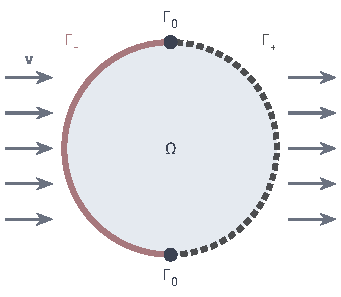
\includegraphics[width=57.8mm]{figures/06-differential-equations/02-partial-differential-equations/tikz/transp-boundary-parts/figure.pdf}
  \caption{速度场$\bm{v}=(1,0)^{\top}$（灰色箭头）下，圆盘的边界分成三部分：红色实线是入流边界$\Gamma_{-}$，深灰虚线是出流边界$\Gamma_{+}$，上下两点是$\bm{v}\cdot\bm{n}=0$的$\Gamma_{0}$。}
  \label{fig:transp-boundary-parts}
\end{BookInlineFigure}

下面在$(0,1)$上取$\rho_0=1$，看三个例子，$M(0)=1$。

第一，$v=1$，$g=0$。这时$\rho(x,t)=1$（$x>t$）、$\rho=0$（$x<t$）。质量以单位速率从右端流出，所以
\[
  M(t)=\max\{1-t,\ 0\}.
\]
式~\eqref{eq:transp-mass-rate}的流出项在$t<1$时等于$\rho(1,t)\cdot1=1$，符合$M'=-1$。

第二，$v=x-1/2$，两端都是出流。解是$\rho=\mathrm{e}^{-t}$，代入验证：
\[
  \partial_t\rho=-\mathrm{e}^{-t},\qquad \partial_x\bigl(\rho\,(x-\tfrac12)\bigr)=\mathrm{e}^{-t}.
\]
两端的流出量都是$\tfrac12\mathrm{e}^{-t}$，合起来恰好是$M'=-\mathrm{e}^{-t}$，因此
\[
  M(t)=\mathrm{e}^{-t}.
\]

第三，$v=x(1-x)$，两端$v=0$，边界是无通量的。例~\ref{ex:transp-logistic-density}中质量向右端堆积，但始终没有离开区间，
\[
  M(t)=1.
\]

这三种情形对应图~\ref{fig:transp-mass-balance}。把第一例换成$g=2$，则$t<1$时左端流入$2$、右端流出$1$，$M=1+t$；$t\geq1$时整个区间密度为$2$，进出相等，$M=2$。

\begin{BookInlineFigure}
  \centering
  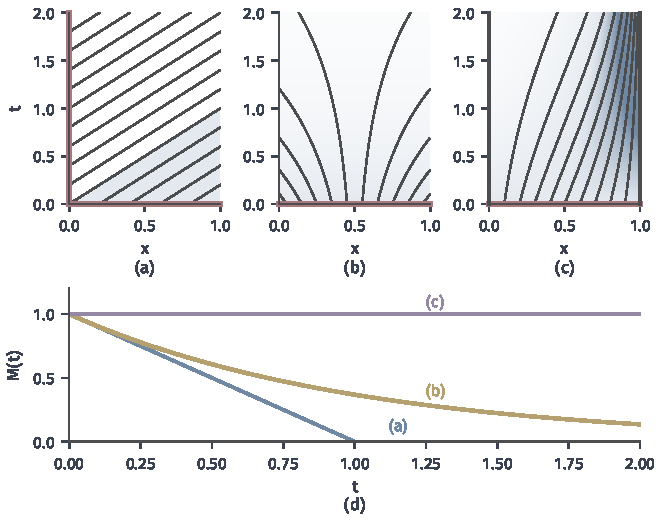
\includegraphics[width=112mm]{figures/06-differential-equations/02-partial-differential-equations/matplotlib/transp-mass-balance/figure.pdf}
  \caption{$(0,1)$上的质量平衡，$\rho_0=1$。上排是特征线（深灰）和密度（蓝色越深越大）：(a)$v=1$，入流数据为$0$；(b)$v=x-1/2$，两端出流；(c)$v=x(1-x)$，两端无通量（粗线）。红线是给数据的边界。(d)三种情形的总质量$M(t)$。}
  \label{fig:transp-mass-balance}
\end{BookInlineFigure}

质量守恒是一个有条件的结论。只有当右端全部为零时，$M$才不变，典型条件是$\Omega$封闭，即$\partial\Omega$上$\bm{v}\cdot\bm{n}=0$，并且没有源项。此时轨迹不会穿过边界，流映射把$\Omega$映到自身，定理~\ref{thm:transp-density}的论证可以在$\Omega$上进行，例~\ref{ex:transp-logistic-density}就是这样。否则，全空间上的守恒结论不能照搬到有界区域。

\section{弱形式}
\label{sec:transp-weak}

三角形初值有折角，台阶初值有跳跃，这些初值都没有经典解的资格，可是特征线公式照样给出了合理的函数。怎样说它们“满足方程”？第~\ref{chap:pde-problems}章的办法是把导数转移到测试函数上。输运方程和连续性方程的导数位置不同，转移之后的结果也不同，所以要分别处理。

下面取$\Omega=\mathbb{R}^{d}$，设$\bm{v}$满足条件（V），测试函数$\psi\in C^{1}_{c}(\mathbb{R}^{d}\times[0,T))$，它在$t=T$附近为零，在$t=0$可以不为零。

\paragraph{两个弱形式}
设$u$是输运方程的经典解。乘以$\psi$，在$\mathbb{R}^{d}\times(0,T)$上积分。时间项对$t$分部积分，产生初值的边界项；空间项写成$\psi\bm{v}\cdot\nabla u$，对$\bm{x}$分部积分，导数要落到$\psi\bm{v}$上。

得到的关系里不再有$u$的导数，只有$\psi\bm{v}$的散度
\[
  \nabla\cdot(\psi\bm{v})=\bm{v}\cdot\nabla\psi+\psi\,\nabla\cdot\bm{v}.
\]

连续性方程的空间项本来就是散度，分部积分后导数只落在$\psi$上，$\bm{v}$不被求导。

\begin{definition}[输运方程与连续性方程的弱解]
\label{def:transp-weak}
设$u_0,\rho_0\in L^{1}_{\mathrm{loc}}(\mathbb{R}^{d})$，$f\in L^{1}_{\mathrm{loc}}(\mathbb{R}^{d}\times[0,T))$。称$u\in L^{1}_{\mathrm{loc}}(\mathbb{R}^{d}\times[0,T))$是输运方程的弱解，若对所有测试函数$\psi$，有
\begin{equation}
  \int_0^{T}\!\!\int u\bigl(\partial_t\psi+\nabla\cdot(\psi\bm{v})\bigr)\,\mathrm{d}\bm{x}\,\mathrm{d}t
  +\int u_0\,\psi(\cdot,0)\,\mathrm{d}\bm{x}
  +\int_0^{T}\!\!\int f\psi\,\mathrm{d}\bm{x}\,\mathrm{d}t=0.
  \label{eq:transp-weak-transport}
\end{equation}
称$\rho\in L^{1}_{\mathrm{loc}}(\mathbb{R}^{d}\times[0,T))$是连续性方程的弱解，若对所有测试函数$\psi$，有
\begin{equation}
  \int_0^{T}\!\!\int\rho\bigl(\partial_t\psi+\bm{v}\cdot\nabla\psi\bigr)\,\mathrm{d}\bm{x}\,\mathrm{d}t
  +\int\rho_0\,\psi(\cdot,0)\,\mathrm{d}\bm{x}
  +\int_0^{T}\!\!\int f\psi\,\mathrm{d}\bm{x}\,\mathrm{d}t=0.
  \label{eq:transp-weak-continuity}
\end{equation}
\end{definition}

两式都不含未知函数的导数，所以间断函数也可以代入。对比可以发现，式~\eqref{eq:transp-weak-transport}中出现了$\nabla\cdot\bm{v}$，要求速度场的散度是函数；式~\eqref{eq:transp-weak-continuity}只需要$\rho\bm{v}$局部可积，对$\bm{v}$的要求弱得多。

分部积分的步骤可逆，所以当$u$或$\rho$是$C^{1}$函数时，弱解就是经典解。下面用一个例子看看弱形式如何辨别间断的传播速度。

\begin{example}[台阶的传播速度]
\label{ex:transp-step}
取一维$v=1$，$f=0$，台阶初值$u_0=1$（$x<0$）、$u_0=0$（$x>0$）。考虑以速度$s>0$移动的台阶$u_s=1$（$x<st$）、$u_s=0$（$x>st$）。

把$u_s$代入式~\eqref{eq:transp-weak-transport}，记左端为$R(s)$，并令$I=\int_0^{T}\psi(st,t)\,\mathrm{d}t$。先算空间项，由微积分基本定理，
\[
  \int_0^{T}\!\!\int_{-\infty}^{st}\partial_x\psi\,\mathrm{d}x\,\mathrm{d}t=I.
\]

再算时间项。积分上限随时间移动，由含参积分的求导法则，
\[
  \frac{\mathrm{d}}{\mathrm{d}t}\int_{-\infty}^{st}\psi\,\mathrm{d}x=\int_{-\infty}^{st}\partial_t\psi\,\mathrm{d}x+s\psi(st,t).
\]
对$t$从$0$到$T$积分，
\[
  \int_0^{T}\!\!\int_{-\infty}^{st}\partial_t\psi\,\mathrm{d}x\,\mathrm{d}t
  =-\int_{-\infty}^{0}\psi(x,0)\,\mathrm{d}x-sI.
\]

两项相加，再加上初值项$\int_{-\infty}^{0}\psi(x,0)\,\mathrm{d}x$，初值积分抵消，
\[
  R(s)=(1-s)\,I.
\]
只要存在使$I\neq0$的测试函数，$R(s)=0$就等价于$s=1$。所以台阶的弱解只能以特征速度$1$移动。
\end{example}

图~\ref{fig:transp-weak-step}(a)的紫色等值线是一个测试函数，它跨在间断线的两侧。(b)用光滑的初值逼近台阶，光滑解$u_0^{\varepsilon}(x-t)$在$\varepsilon\to0$时收敛到台阶解，这也说明台阶解是光滑解的极限。(c)对一个具体的$\psi$计算了$R(s)$，绿点是数值积分的结果，只有$s=1$时为零。

\begin{BookInlineFigure}
  \centering
  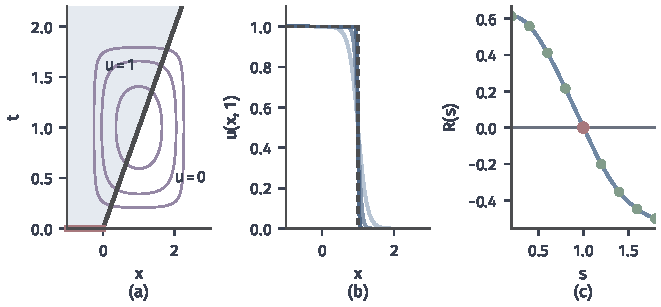
\includegraphics[width=112mm]{figures/06-differential-equations/02-partial-differential-equations/matplotlib/transp-weak-step/figure.pdf}
  \caption{台阶解的弱形式，$v=1$。(a)左侧浅蓝区域$u=1$，深灰粗线是间断线$x=t$，紫色曲线是测试函数$\psi$的等值线，红线是初值$1$的部分。(b)光滑化初值的解在$t=1$的剖面（蓝色由浅到深，过渡带越来越窄），虚线是台阶解。(c)$R(s)=(1-s)\int\psi(st,t)\,\mathrm{d}t$（蓝）与数值积分（绿），红点是$s=1$。}
  \label{fig:transp-weak-step}
\end{BookInlineFigure}

\paragraph{流构造就是弱解}
一般的情形下，第~\ref{sec:transp-flow}节的公式对粗糙的数据仍给出弱解，并且在$\bm{v}$足够正则时它是唯一的。

\begin{theorem}[流构造给出弱解]
\label{thm:transp-weak}
设$\bm{v}$满足条件（V）。
\begin{enumerate}
  \item 对$\rho_0\in L^{1}_{\mathrm{loc}}(\mathbb{R}^{d})$，函数
  \begin{equation}
    \rho(\bm{y},t)=\rho_0\bigl(\bm{\varphi}_{t,0}(\bm{y})\bigr)\,J_{t,0}(\bm{y})
    \label{eq:transp-weak-density}
  \end{equation}
  是连续性方程（$f=0$）的弱解，且是$L^{1}_{\mathrm{loc}}$中唯一的弱解。
  \item 对$u_0\in L^{1}_{\mathrm{loc}}(\mathbb{R}^{d})$，$u=u_0\circ\bm{\varphi}_{t,0}$是输运方程（$f=0$）的弱解。若$\nabla\cdot\bm{v}$还关于$\bm{x}$连续可微，这个弱解是$L^{1}_{\mathrm{loc}}$中唯一的。
\end{enumerate}
\end{theorem}

\begin{proof}
先证$\rho$是弱解。固定$\bm{x}$，由式~\eqref{eq:transp-flow}，沿轨迹有
\[
  \frac{\mathrm{d}}{\mathrm{d}t}\psi\bigl(\bm{\varphi}_{0,t}(\bm{x}),t\bigr)
  =\bigl(\partial_t\psi+\bm{v}\cdot\nabla\psi\bigr)\bigl(\bm{\varphi}_{0,t}(\bm{x}),t\bigr).
\]

在$[0,T]$上积分。$\psi$在$t=T$附近为零，于是
\[
  -\psi(\bm{x},0)=\int_0^{T}\bigl(\partial_t\psi+\bm{v}\cdot\nabla\psi\bigr)\bigl(\bm{\varphi}_{0,t}(\bm{x}),t\bigr)\,\mathrm{d}t.
\]

两边乘以$\rho_0(\bm{x})$，对$\bm{x}$积分并交换积分次序。式~\eqref{eq:transp-weak-density}的$\rho$满足式~\eqref{eq:transp-density}，换元$\bm{y}=\bm{\varphi}_{0,t}(\bm{x})$后，右端正是$\int_0^{T}\!\int\rho(\partial_t\psi+\bm{v}\cdot\nabla\psi)\,\mathrm{d}\bm{y}\,\mathrm{d}t$，这就是式~\eqref{eq:transp-weak-continuity}。

再证$u$是弱解。沿轨迹求导时多带一个因子$J_{0,t}$，由式~\eqref{eq:transp-liouville}，
\[
  \frac{\mathrm{d}}{\mathrm{d}t}\Bigl[\psi\bigl(\bm{\varphi}_{0,t}(\bm{x}),t\bigr)J_{0,t}(\bm{x})\Bigr]
  =\bigl(\partial_t\psi+\nabla\cdot(\psi\bm{v})\bigr)\bigl(\bm{\varphi}_{0,t}(\bm{x}),t\bigr)\,J_{0,t}(\bm{x}).
\]
对$t$积分，初值是$\psi(\bm{x},0)$。乘以$u_0(\bm{x})$，对$\bm{x}$积分，再把$\mathrm{d}\bm{x}$上的$J_{0,t}$用换元吸收，得到式~\eqref{eq:transp-weak-transport}。

接着证连续性方程的唯一性。设$\rho$是$\rho_0=0$的弱解，任取$h\in C^{1}_{c}(\mathbb{R}^{d}\times(0,T))$。定义
\[
  \psi(\bm{x},t)=-\int_t^{T}h\bigl(\bm{\varphi}_{t,r}(\bm{x}),r\bigr)\,\mathrm{d}r.
\]

由式~\eqref{eq:transp-flow-rules}，$\bm{\varphi}_{t,r}$是$\bm{\varphi}_{0,r}$与$\bm{\varphi}_{t,0}$的复合，关于$(\bm{x},t)$是$C^{1}$的，所以$\psi\in C^{1}$。$\psi$在$t=T$附近为零，$h$的支集紧，流映射连续，所以$\psi$的支集也紧，它是合法的测试函数。

任取一条轨迹$\bm{Y}(t)$，由定义，
\[
  \psi\bigl(\bm{Y}(t),t\bigr)=-\int_t^{T}h\bigl(\bm{Y}(r),r\bigr)\,\mathrm{d}r.
\]
对$t$求导，得到
\[
  \partial_t\psi+\bm{v}\cdot\nabla\psi=h.
\]
代入式~\eqref{eq:transp-weak-continuity}，得到
\[
  \int_0^{T}\!\!\int\rho h\,\mathrm{d}\bm{x}\,\mathrm{d}t=0.
\]
这对所有$h$成立，所以$\rho=0$几乎处处成立。

最后证输运方程的唯一性。令$c=\nabla\cdot\bm{v}$，取同样的$h$，定义
\[
  \psi(\bm{x},t)=-\int_t^{T}h\bigl(\bm{\varphi}_{t,r}(\bm{x}),r\bigr)\exp\Bigl(\int_t^{r}c\bigl(\bm{\varphi}_{t,\tau}(\bm{x}),\tau\bigr)\,\mathrm{d}\tau\Bigr)\mathrm{d}r.
\]

$c$关于$\bm{x}$是$C^{1}$的，所以$\psi\in C^{1}$，这就是额外假设的作用。沿轨迹用积分因子，得到$\partial_t\psi+\bm{v}\cdot\nabla\psi+c\psi=h$，即$\partial_t\psi+\nabla\cdot(\psi\bm{v})=h$。代入式~\eqref{eq:transp-weak-transport}，同样推出$u=0$。
\end{proof}

有源项时，解按式~\eqref{eq:transp-flow-solution}和式~\eqref{eq:transp-density-source}叠加，证明的计算相同，唯一性的结论也不变。

这个证明还揭示了两个方程之间的对偶关系。若$u$满足无源输运方程、$\rho$满足无源连续性方程，且二者足够光滑、衰减足够快，那么直接求导，用分部积分，可得
\[
  \frac{\mathrm{d}}{\mathrm{d}t}\int\rho u\,\mathrm{d}\bm{x}
  =\int\bigl(u\,\partial_t\rho+\rho\,\partial_tu\bigr)\,\mathrm{d}\bm{x}
  =\int\bigl(-u\nabla\cdot(\rho\bm{v})-\rho\bm{v}\cdot\nabla u\bigr)\,\mathrm{d}\bm{x}=0.
\]
也就是说，质量加权的标签总量不随时间变化。$h$与$\psi$的构造正是在利用这一点。

\paragraph{测度形式}
由于式~\eqref{eq:transp-weak-continuity}中不含$\bm{v}$的导数，也可以让$\rho_0$是测度。把积分$\int\rho_0\psi\,\mathrm{d}\bm{x}$换成$\int\psi\,\mathrm{d}\mu_0$，就可以描述集中在一点的质量。

取$\mu_0=\delta_{\bm{x}_0}$，式~\eqref{eq:transp-pushforward-measure}给出$\mu_t=\delta_{\bm{\varphi}_{0,t}(\bm{x}_0)}$，这个Dirac质量跟着粒子走。这是第~\ref{sec:transp-continuity}节密度搬运的极端情形，此时密度不再是函数，但质量守恒和推前关系仍然成立。

\paragraph{粗糙速度场}
以上结论都建立在条件（V）上。把$\bm{v}$换成粗糙的场，弱形式的写法没有变化，定理~\ref{thm:transp-weak}的结论却可能失效。

看图~\ref{fig:transp-rough-velocity}中的两个间断速度场。(a)$v=-\mathrm{sgn}(x)$：粒子从两侧撞向原点。$\rho_0=1$（$\lvert x\rvert<1$）时，$t<1$时的质量分布是
\begin{equation}
  \mu_t=\mathbf{1}_{\lvert x\rvert<1-t}\,\mathrm{d}x+2t\,\delta_0.
  \label{eq:transp-collision}
\end{equation}
质量在原点集中成Dirac，不再是函数。$\delta_0$处还需要规定$v$的取值，式~\eqref{eq:transp-collision}用的是$v(0)=0$，这个零测集上的取值现在影响结论。

(b)$v=\mathrm{sgn}(x)$：粒子从原点向两侧分开，$\lvert x\rvert<t$形成一块没有粒子来过的区域，浅红色部分。对输运方程来说，这里的值没有被初值决定。

对连续性方程，唯一性也会失败。看(c)：取$v=\mathrm{sgn}(x)$，初值$\rho_0=0$，定义
\begin{equation}
  \rho(x,t)=
  \begin{cases}
    t-x, & 0<x<t,\\
    -(t+x), & -t<x<0,\\
    0, & \text{其他}.
  \end{cases}
  \label{eq:transp-nonunique-density}
\end{equation}

\begin{BookInlineFigure}
  \centering
  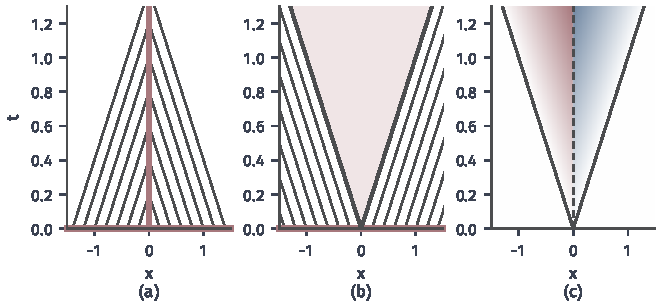
\includegraphics[width=112mm]{figures/06-differential-equations/02-partial-differential-equations/matplotlib/transp-rough-velocity/figure.pdf}
  \caption{间断速度场的三种问题，红线在(a)(b)中是初始线。(a)$v=-\mathrm{sgn}(x)$，特征线（深灰）撞向原点，红色粗线处积累质量。(b)$v=\mathrm{sgn}(x)$，浅红区域没有特征线到达。(c)$v=\mathrm{sgn}(x)$、$\rho_0=0$时的非零弱解~\eqref{eq:transp-nonunique-density}，红—白—蓝色阶的中点为$0$。}
  \label{fig:transp-rough-velocity}
\end{BookInlineFigure}

验证如下。在$x>0$的一侧，$v=1$，$\rho=t-x$满足$\partial_t\rho+\partial_x\rho=1-1=0$；$x<0$一侧，$v=-1$，$\rho=-(t+x)$满足$\partial_t\rho-\partial_x\rho=-1+1=0$。在分界线$x=0$上，右侧流量$\rho v=t\cdot1=t$，左侧流量$(-t)\cdot(-1)=t$，两侧相等，所以弱形式成立。

沿$x=\pm t$，$\rho$连续，没有问题。于是初值为零的问题有非零弱解，弱解在这里不唯一。式~\eqref{eq:transp-nonunique-density}的$\rho$有正有负，它在$x=0$两侧同时“产生”正、负质量。

这些例子都说明，弱形式并不会自动带来好的理论。超出Lipschitz范围的速度场需要专门的工具，结论依赖于$\nabla\bm{v}$的Sobolev型正则性和散度的有界性，这已超出本章的范围。本章的结论不能自动推广到任意粗糙的速度场。

\paragraph{有界区域上的弱形式}
有界区域的连续性方程也有相应的写法。要把$\Gamma_{-}$上的入流数据$g$放进去，测试函数应在$\Gamma_{+}$上为零。乘以$\psi$后分部积分，得到
\begin{equation}
  \int_0^{T}\!\!\int_{\Omega}\rho\bigl(\partial_t\psi+\bm{v}\cdot\nabla\psi\bigr)\,\mathrm{d}\bm{x}\,\mathrm{d}t
  +\int_{\Omega}\rho_0\psi(\cdot,0)\,\mathrm{d}\bm{x}
  +\int_0^{T}\!\!\int_{\Gamma_{-}}g\,\lvert\bm{v}\cdot\bm{n}\rvert\,\psi\,\mathrm{d}S\,\mathrm{d}t=0.
  \label{eq:transp-weak-boundary}
\end{equation}
边界项与式~\eqref{eq:transp-mass-rate}的入流项相对应，$\Gamma_{+}$上$\psi=0$让未知的出流值不进入方程。

\section{数据稳定性}
\label{sec:transp-stability}

测量得到的初值、源项和速度场总有误差。这些误差会被放大多少？答案与所用的范数有关，也与误差出现在哪个量上有关。

\paragraph{数据误差的$L^p$估计}
输运方程对$u$是线性的，同一速度场下，两个解的差$e$满足同一方程，其初值和源项分别是初值之差$e_0$与源项之差$g_e$。所以只需估计式~\eqref{eq:transp-flow-solution}给出的$e$。

要点是：逆流映射$\bm{\varphi}_{t,s}$的复合不改变函数的最大值，但会改变$L^{p}$范数，因为积分时要换元。这时$J_{s,t}$进入估计。

\begin{theorem}[数据误差的$L^{p}$估计]
\label{thm:transp-lp}
设$\bm{v}$满足条件（V），存在常数$\kappa\geq0$使$\nabla\cdot\bm{v}\leq\kappa$。设$1\leq p<\infty$，$e_0\in L^{p}(\mathbb{R}^{d})$，$g_e\in L^{1}(0,T;L^{p}(\mathbb{R}^{d}))$，$e$由式~\eqref{eq:transp-flow-solution}给出。则对$t\in[0,T]$，
\begin{equation}
  \lVert e(\cdot,t)\rVert_{p}\leq\mathrm{e}^{\kappa t/p}\lVert e_0\rVert_{p}
  +\int_0^{t}\mathrm{e}^{\kappa(t-s)/p}\lVert g_e(\cdot,s)\rVert_{p}\,\mathrm{d}s.
  \label{eq:transp-lp-estimate}
\end{equation}
当$e_0\in L^{\infty}$，$g_e\in L^{1}(0,T;L^{\infty})$时，把上式中的$\mathrm{e}^{\kappa\cdot/p}$换成$1$，无需假设散度有上界，结论对$p=\infty$成立。
\end{theorem}

\begin{proof}
先看单个函数的复合。设$w\in L^{p}$，换元$\bm{y}=\bm{\varphi}_{t,s}(\bm{x})$，即$\bm{x}=\bm{\varphi}_{s,t}(\bm{y})$，体积元多出因子$J_{s,t}(\bm{y})$，得到
\[
  \int\bigl\lvert w\bigl(\bm{\varphi}_{t,s}(\bm{x})\bigr)\bigr\rvert^{p}\,\mathrm{d}\bm{x}
  =\int\lvert w(\bm{y})\rvert^{p}J_{s,t}(\bm{y})\,\mathrm{d}\bm{y}.
\]

由式~\eqref{eq:transp-liouville-solution}和$\nabla\cdot\bm{v}\leq\kappa$，$J_{s,t}\leq\mathrm{e}^{\kappa(t-s)}$。开$p$次方，
\[
  \lVert w\circ\bm{\varphi}_{t,s}\rVert_{p}\leq\mathrm{e}^{\kappa(t-s)/p}\lVert w\rVert_{p}.
\]

把这个估计用于式~\eqref{eq:transp-flow-solution}的第一项，以及第二项中被积函数的$L^p$范数，再用Minkowski积分不等式把范数移入积分号，就得到式~\eqref{eq:transp-lp-estimate}。对$p=\infty$，复合映射双射，本性上确界不变，同样的步骤给出结论，$J$不再出现。
\end{proof}

式~\eqref{eq:transp-lp-estimate}表明，放大来自局部的体积膨胀：$p$越大，因子$\mathrm{e}^{\kappa t/p}$越接近$1$，$p=\infty$时不放大。

对例~\ref{ex:transp-stretch}的$v=x$，有$\kappa=1$，$J_{0,t}=\mathrm{e}^{t}$是常数。此时$e(x,t)=e_0(x\mathrm{e}^{-t})$，换元得到精确的等式：
\begin{equation}
  \lVert e(\cdot,t)\rVert_{p}=\mathrm{e}^{t/p}\lVert e_0\rVert_{p},
  \label{eq:transp-lp-example}
\end{equation}
所以式~\eqref{eq:transp-lp-estimate}中的因子不能再改进。

密度的情形相反。$\rho$按式~\eqref{eq:transp-density}搬运时，换元给出
\begin{equation}
  \lVert\rho(\cdot,t)\rVert_{p}^{p}=\int\lvert\rho_0(\bm{x})\rvert^{p}\,J_{0,t}(\bm{x})^{1-p}\,\mathrm{d}\bm{x}.
  \label{eq:transp-density-lp}
\end{equation}
$p=1$时$J$的幂次为零，$L^{1}$范数不变，这是质量守恒的范数形式。$p>1$时，密度的误差在压缩处被放大，在膨胀处被缩小，放大倍数由$\inf J_{0,t}$控制。

图~\ref{fig:transp-stability-lp}比较了$v=x$下三角形误差的范数，(a)是$u$的误差，(b)是$\rho$的误差。$u$的$L^{1}$误差增长最快，$L^{\infty}$不变；$\rho$恰好反过来，$L^{1}$不变，$L^{\infty}$衰减最快。线是精确的指数公式，绿点是数值积分。

\begin{BookInlineFigure}
  \centering
  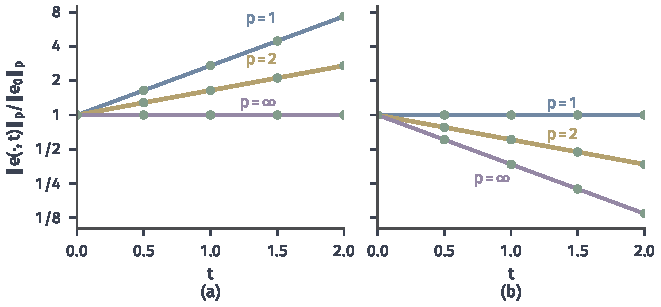
\includegraphics[width=112mm]{figures/06-differential-equations/02-partial-differential-equations/matplotlib/transp-stability-lp/figure.pdf}
  \caption{速度场$v=x$下误差范数的变化（纵轴为对数），$p=1,2,\infty$依次为蓝、黄、紫，绿点是用数值积分算出的范数比。(a)场值误差，满足式~\eqref{eq:transp-lp-example}。(b)密度误差，因子为$\mathrm{e}^{-(1-1/p)t}$。}
  \label{fig:transp-stability-lp}
\end{BookInlineFigure}

\paragraph{比较两个速度场}
现在让速度场本身有误差，初值和源项相同。上面的线性结构用不上了，因为$u^{a}$与$u^{b}$沿不同的轨迹搬运。此时的思路是比较两组特征线，再用数据的空间Lipschitz常数把轨迹差转换为场值差。

\begin{theorem}[速度场误差的$L^{\infty}$估计]
\label{thm:transp-velocity}
设$\bm{v}^{a},\bm{v}^{b}$满足条件（V），其中$\bm{v}^{a}$的常数为$L$，并存在可积函数$\delta$，使
\begin{equation}
  \lVert\bm{v}^{a}(\bm{x},t)-\bm{v}^{b}(\bm{x},t)\rVert_2\leq\delta(t).
  \label{eq:transp-velocity-gap}
\end{equation}
设$u_0$是$L_0$-Lipschitz函数，$f(\cdot,s)$是$L_f$-Lipschitz函数（常数不依赖$s$）。令$u^{a},u^{b}$分别是由式~\eqref{eq:transp-flow-solution}给出的解，定义
\begin{equation}
  E(t,s)=\int_s^{t}\mathrm{e}^{L(r-s)}\delta(r)\,\mathrm{d}r.
  \label{eq:transp-velocity-integral}
\end{equation}
则
\begin{equation}
  \lVert u^{a}(\cdot,t)-u^{b}(\cdot,t)\rVert_{\infty}
  \leq L_0\,E(t,0)+L_f\int_0^{t}E(t,s)\,\mathrm{d}s.
  \label{eq:transp-velocity-estimate}
\end{equation}
\end{theorem}

\begin{proof}
固定$\bm{x}$和$t$，令$\bm{x}^{a}(r)=\bm{\varphi}^{a}_{t,r}(\bm{x})$，$\bm{x}^{b}$同理，$z(r)=\lVert\bm{x}^{a}(r)-\bm{x}^{b}(r)\rVert_2$。两条曲线在$r=t$处重合，从$r$到$t$积分两者的差，
\[
  \bm{x}^{a}(r)-\bm{x}^{b}(r)
  =-\int_r^{t}\bigl(\bm{v}^{a}(\bm{x}^{a},\tau)-\bm{v}^{b}(\bm{x}^{b},\tau)\bigr)\,\mathrm{d}\tau.
\]

在被积函数中加减$\bm{v}^{a}(\bm{x}^{b},\tau)$，第一组差用$L$，第二组差用$\delta$，于是
\[
  z(r)\leq Z(r):=\int_r^{t}\bigl(Lz(\tau)+\delta(\tau)\bigr)\,\mathrm{d}\tau.
\]

由$-Z'(r)=Lz+\delta\leq LZ+\delta$，乘以积分因子，
\[
  \frac{\mathrm{d}}{\mathrm{d}r}\Bigl[\mathrm{e}^{L(r-s)}Z(r)\Bigr]
  =\mathrm{e}^{L(r-s)}\bigl(LZ(r)+Z'(r)\bigr)\geq-\mathrm{e}^{L(r-s)}\delta(r).
\]

从$s$到$t$积分，并用$Z(t)=0$，
\[
  z(s)\leq Z(s)\leq\int_s^{t}\mathrm{e}^{L(r-s)}\delta(r)\,\mathrm{d}r=E(t,s).
\]

这是反向的Gronwall估计，相当于第~\ref{chap:ode-sensitivity}章的结论在时间翻转下的形式。把它代入式~\eqref{eq:transp-flow-solution}，两项分别用$u_0$和$f(\cdot,s)$的Lipschitz常数控制，就得到式~\eqref{eq:transp-velocity-estimate}。
\end{proof}

式~\eqref{eq:transp-velocity-estimate}中$E$的指数因子和$\delta$的时间积分都有明确的含义：时刻$r$的速度误差造成轨迹偏差，沿着剩余的时间由流的拉伸放大，再由数据的斜率转化为场值误差。

取$\bm{v}^{a}=1$，$\bm{v}^{b}=1+\delta$，$f=0$，初值是以$0$为中心、半宽为$1$的三角形。此时$L=0$，$L_0=1$，$E(t,0)=\delta t$，估计给出$\lVert u^{a}-u^{b}\rVert_{\infty}\leq\delta t$。当$\delta t\leq1$时，这恰好是解的实际差：两个三角形错开$\delta t$，在斜边上的差就是$\delta t$。$\delta=0.2$，$t=1.5$时差为$0.3$。

\paragraph{间断初值}
初值有间断时，式~\eqref{eq:transp-velocity-estimate}中的$L_0$是无穷大，估计完全失效。台阶初值$u_0=\mathbf{1}_{x<0}$在$v=1$与$v=1+\delta$下的解，只要$\delta>0$、$t>0$，就总存在宽度为$\delta t$的一段，两解相差$1$，所以
\begin{equation}
  \lVert u^{a}(\cdot,t)-u^{b}(\cdot,t)\rVert_{\infty}=1.
  \label{eq:transp-step-sup}
\end{equation}
一致范数下解对速度场不连续。积分范数则仍然能捕捉到这段宽度的微小：
\begin{equation}
  \lVert u^{a}(\cdot,t)-u^{b}(\cdot,t)\rVert_{p}=(\delta t)^{1/p},\qquad 1\leq p<\infty.
  \label{eq:transp-step-lp}
\end{equation}

图~\ref{fig:transp-velocity-perturb}对比了两种初值。(a)中平滑的三角形错开一点点，差也很小，(b)中台阶错开任意小，最大差都是$1$，但差的区域宽度很窄。(c)把这几个量对$\delta$作图。

\begin{BookInlineFigure}
  \centering
  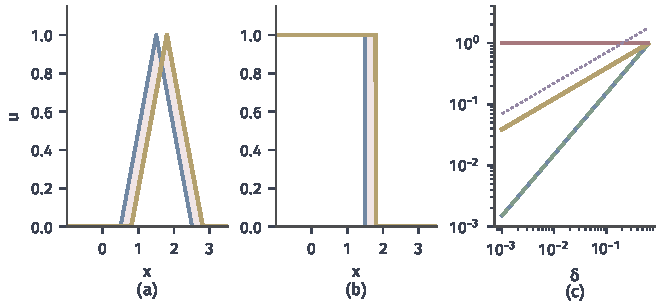
\includegraphics[width=112mm]{figures/06-differential-equations/02-partial-differential-equations/matplotlib/transp-velocity-perturb/figure.pdf}
  \caption{$v=1$（蓝）与$v=1+\delta$（黄）的解，$t=1.5$，$\delta=0.2$，浅红区域是两解的差。(a)三角形初值。(b)台阶初值。(c)误差随$\delta$的变化（对数坐标）：蓝线是三角形的一致误差，与绿色虚线（台阶的$L^{1}$误差）重合，都正比于$\delta$；黄线是台阶的$L^{2}$误差，与紫色点线（参考斜率$1/2$）平行；红线是台阶的一致误差。}
  \label{fig:transp-velocity-perturb}
\end{BookInlineFigure}

式~\eqref{eq:transp-step-lp}的收敛率$1/p$比光滑情形的一阶要慢，$p=2$时只有$1/2$阶。对一般的$L^{p}$初值，收敛仍然成立，只是不再有统一的速率。

\begin{theorem}[粗糙初值的$L^{p}$收敛]
\label{thm:transp-lp-convergence}
设$\bm{v}^{n},\bm{v}$满足条件（V），常数$L$相同，$\nabla\cdot\bm{v}^{n},\nabla\cdot\bm{v}\leq\kappa$，且$\bm{v}^{n}$在$\mathbb{R}^{d}\times[0,T]$上一致收敛于$\bm{v}$。设$u_0\in L^{p}(\mathbb{R}^{d})$，$1\leq p<\infty$，$u^{n},u$是相应的解$u_0\circ\bm{\varphi}^{n}_{t,0}$与$u_0\circ\bm{\varphi}_{t,0}$。则对每个$t\in[0,T]$，
\begin{equation}
  \lVert u^{n}(\cdot,t)-u(\cdot,t)\rVert_{p}\to0.
  \label{eq:transp-lp-convergence}
\end{equation}
\end{theorem}

\begin{proof}
任取$\varepsilon>0$。Lipschitz紧支函数在$L^{p}$中稠密，取这样的$w$，使$\lVert u_0-w\rVert_{p}<\varepsilon$，它的支集在球$B$内，Lipschitz常数为$L_w$。三角不等式给出
\[
  \lVert u^{n}-u\rVert_{p}\leq\lVert(u_0-w)\circ\bm{\varphi}^{n}_{t,0}\rVert_{p}
  +\lVert w\circ\bm{\varphi}^{n}_{t,0}-w\circ\bm{\varphi}_{t,0}\rVert_{p}
  +\lVert(w-u_0)\circ\bm{\varphi}_{t,0}\rVert_{p}.
\]

由定理~\ref{thm:transp-lp}的证明，第一项和第三项都不超过$\mathrm{e}^{\kappa t/p}\varepsilon$。第二项中，定理~\ref{thm:transp-velocity}的第一步给出逐点差不超过$L_wE_n$，其中$E_n\to0$。

被积函数只在$\bm{\varphi}^{n}_{0,t}(B)\cup\bm{\varphi}_{0,t}(B)$上非零，这个集合的体积不超过$2\mathrm{e}^{\kappa t}\lvert B\rvert$，所以第二项不超过
\[
  L_wE_n\bigl(2\mathrm{e}^{\kappa t}\lvert B\rvert\bigr)^{1/p}\to0.
\]
先让$n\to\infty$，再让$\varepsilon\to0$，即得式~\eqref{eq:transp-lp-convergence}。
\end{proof}

定理中$p<\infty$是必需的：式~\eqref{eq:transp-step-sup}就是$p=\infty$的反例。$\varepsilon$的取法依赖$u_0$，所以这里没有速率，这也是间断初值与Lipschitz初值的根本差别。

\paragraph{弱收敛}
数据本身的扰动也可能只在弱意义下小。比如$u_0^{n}(x)=\sin(nx)$在$L^{2}$的有界区间上弱收敛于$0$，但它的$L^{2}$范数不趋于零。

固定速度场，$u_0^{n}\rightharpoonup u_0$（$L^{p}$中弱收敛，$1<p<\infty$）时，对任意$h\in C_c(\mathbb{R}^{d})$，由换元，
\[
  \int u^{n}(\bm{y},t)h(\bm{y})\,\mathrm{d}\bm{y}
  =\int u_0^{n}(\bm{x})\,h\bigl(\bm{\varphi}_{0,t}(\bm{x})\bigr)J_{0,t}(\bm{x})\,\mathrm{d}\bm{x}.
\]

右端的$h(\bm{\varphi}_{0,t}(\cdot))J_{0,t}$是一个固定的$L^{p'}$函数，所以它收敛到对应$u_0$的值。这说明解的弱收敛可以从初值传递过来，但它不提供任何一致的误差估计。上面的振荡初值在$v=x$下的解是$\sin(nx\mathrm{e}^{-t})$，它的振幅始终是$1$，只是积分平均趋于零。

\section{本章小结}
\label{sec:transp-summary}

本章从一个问题出发：给定速度场，一滴墨水此后会怎样？答案取决于要问的量。若问粒子携带的值，它沿轨迹不变；若问单位体积的质量，它要除以流动带来的体积倍率。

两种量都通过同一组对象计算。轨迹由常微分方程$\dot{\bm{x}}=\bm{v}(\bm{x},t)$给出，把所有轨迹放在一起得到流映射$\bm{\varphi}_{s,t}$。场值的解是初值与逆流映射的复合，加上沿轨迹累积的源项；密度的解还要多除一个Jacobian行列式$J_{0,t}$，它由速度的散度沿轨迹积分得到。表~\ref{tab:transp-value-density}给出了两者的对比。

这些结论都有明确的条件。

\begin{itemize}
  \item 条件（V）保证了过每一点恰有一条特征线，逆映射在全空间存在。轨迹爆炸时，解只在流映射的值域上有定义；轨迹不唯一时，反向追踪的结果不确定，$C^{1}$解可能不存在。
  \item 总质量守恒需要闭区域、无源项，或全空间上足够的衰减。沿轨迹的密度不变是另一个结论，它只在无散度时成立。
  \item 经典解要求初值$C^{1}$，连续性方程的经典解还要求$\nabla\cdot\bm{v}$对$\bm{x}$连续可微。折角和间断用弱形式处理，弱形式下的存在和唯一仍然要靠条件（V），粗糙速度场下可能出现集中或非唯一。
  \item 数据误差的$L^{p}$放大由体积膨胀控制，速度误差的$L^{\infty}$估计需要初值和源项的Lipschitz常数。间断初值下一致估计失效，只能用$L^{p}$或弱收敛的语言。
\end{itemize}

这一切都有一个共同的前提：速度场是事先给定的，特征线彼此不相交。若传播速度依赖未知量本身，不同高度的点走得快慢不同，特征线就可能相交，解在有限时间内失去光滑性。第~\ref{chap:scalar-conservation-laws}章讨论这种情形。

